\section{Data Analysis}
\label{chap:analysis}

\subsection{Introduction}

This chapter treats of the analysis of the data taken in CLAS for the 
experiments E-02-104 \cite{Brooks:2002aa} and E-02-110 \cite{Hafidi:2002aa}.
The code name for the run is {\it eg2}, it was composed of three phases 
labeled {\it a}, {\it b} and {\it c}. The analysis is performed on the data 
collected in the beginning of 2004 during the third phase ({\it eg2c}), for 
which the beam energy was 5.014 GeV\footnote{The other phases gave a small 
amount of data at a beam energy of 4 GeV.}.

As the two experiments, running simultaneously, aimed at comparing deuterium 
with heavier nuclei, it was decided to use a double target system 
\cite{Hakobyan:2008zz}. The first target is filled with liquid deuterium and 
the second is a solid target. The latter can be made of carbon, aluminum, 
iron, tin or lead and changed remotely (the system is shown in figure 
\ref{fig:phototarget}). The two targets are separated by only 4~cm in order to reduce
the acceptance differences between them. The 
advantage to have the two targets in the beam line simultaneously
is that several systematic effects related to the beam 
and detector properties will cancel in the nuclear ratio.

\begin{figure}[htbp]
\centering
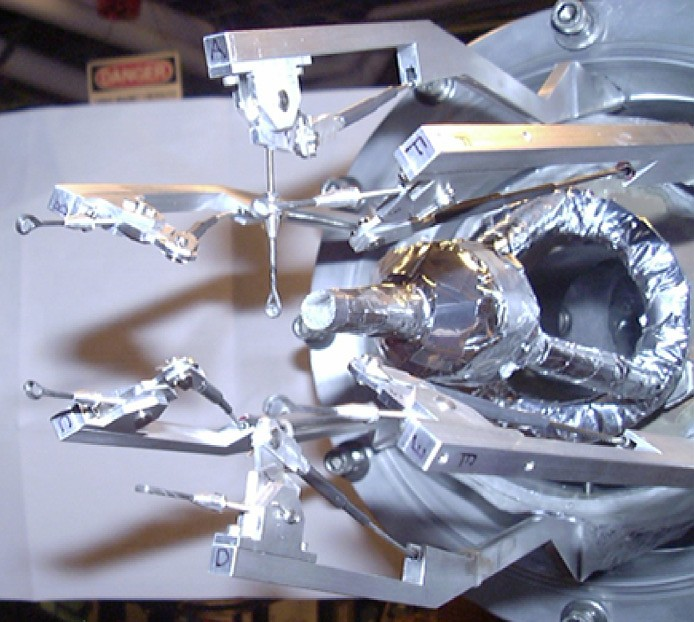
\includegraphics[width=7cm] {chap5-fig/PhTar.jpg} 
\caption {Picture of the target system of the {\it eg2} run. The cryogenic target is 
in the back, enveloped in aluminum foils. The solid targets are held by mechanical arms
allowing to change targets remotely, in the picture the top arm is in the beam line.}
\label{fig:phototarget}
\end{figure}

The analysis of the experiment E-02-110, focusing on the study of color 
transparency effects, has been approved recently \cite{ElFassi:2008}. As this 
analysis went through a careful review by the CLAS collaboration, we use
similar analysis methods when possible. In particular, the electron selection 
presented here is very similar to theirs; the main difference being a new 
target determination method.

In the section \ref{sec:pid}, we identify the following particles e$^-$, 
$\pi^-$ and $\pi^+$ using a series of cuts on the various 
detector outputs. For pions, we use the signal in the drift chambers (DC) and 
in the scintillator counters (SC), for which we require a positive status (global and DC) 
from the reconstruction code. For electron identification, we use signals from 
all detector parts DC, Cherenkov Counters (CC), SC and Electromagnetic 
Calorimeter (EC).

Once particles are identified, we can extract the observables (multiplicity 
ratio and transverse momentum broadening). The method is presented in the 
section \ref{sec:obs}, however these need several corrections presented in the 
section \ref{sec:corrections}. The 
two main corrections are the acceptance of the detector and the radiative 
effects, both are evaluated using Monte-Carlo generator. The evaluation of 
the systematic errors is presented in the section \ref{sec:TotSys}.
The analysis' final results are presented and discussed in the next chapter.

\subsection{Particle Identification}
\label{sec:pid}

\subsubsection{Electron Identification}

First, we apply a fiducial cut on the EC to remove the electrons detected on 
the edge of the calorimeter ($U_{EC}>40$~cm, $V_{EC}<360$~cm and 
$W_{EC}<395$~cm in the calorimeter's coordinates). These are problematic hits 
because the generated electromagnetic shower might be partly outside the 
detector, leading to a wrong measurement of the energy deposited.

To reject pions, we apply cuts on the energy deposited
in the EC using the measurements in the inner ($E_{in}$) and the 
outer part ($E_{out})$ of the calorimeter:

\begin{equation}
\label{einout}
\mu  \left[1-\frac{0.3}{\sqrt{a}}\right] - \frac{E_{in}}{p} \leq 
\frac{E_{out}}{p} \leq 
\mu  \left[1+\frac{0.3}{\sqrt{b}}\right] - \frac{E_{in}}{p},
\end{equation}

where $\mu = 0.271$ is the mean of the fraction of the energy deposited in the 
calorimeter by electrons, the $a$ parameter is set at 0.5 and the parameter 
$b$ is a function of momentum given in table \ref{tab:ecoutin-par}. The 
adjustment of $b$ is motivated by the non-linear dependence of the energy 
deposited as a function of the particle's momentum (see figure \ref{eleEC}). As pions are 
minimum ionizing particles, they are expected to lose a constant energy in 
the inner part of the calorimeter (around 30~MeV), regardless of their 
momentum. Therefore, by requesting more than 60~MeV to be deposited, we 
efficiently cut the pion contamination (see figure~\ref{eleECi}).

\begin{table}[tbp]
  \centering
  \begin{tabular}{@{} cc @{}}
    \hline
    Momentum bin (GeV/c)& Parameter b \\ 
    \hline
    0.5 - 0.7 & 0.85 \\
    0.7 - 0.9 & 0.8  \\
    0.9 - 1.1 & 0.85 \\
    1.1 - 1.3 & 1.05 \\
    1.3 - 1.5 & 1.1  \\
    1.5 - 1.7 & 1.35 \\
    1.7 - 1.9 & 1.35 \\
    1.9 - 2.1 & 1.45 \\
    2.1 - 2.3 & 1.35 \\
    2.3 - 2.5 & 1.35 \\
    2.5 - 2.7 & 1.35 \\
    2.7 - 2.9 & 1.3  \\
    2.9 - 3.1 & 1.35 \\
    3.1 - 3.3 & 1.35 \\
    3.3 - 3.5 & 1.5  \\
    3.5 - 3.7 & 1.6  \\
    3.7 - 3.9 & 1.8  \\
    3.9 - 4.1 & 1.8  \\
    4.1 - 4.3 & 1.8  \\
    4.3 - 4.5 & 1.8  \\
    \hline
  \end{tabular}
  \caption{Values of the parameter $b$ used in equation \ref{einout} for 
           different momentum ranges.}
  \label{tab:ecoutin-par}
\end{table}

\begin{figure}[p]
\centering
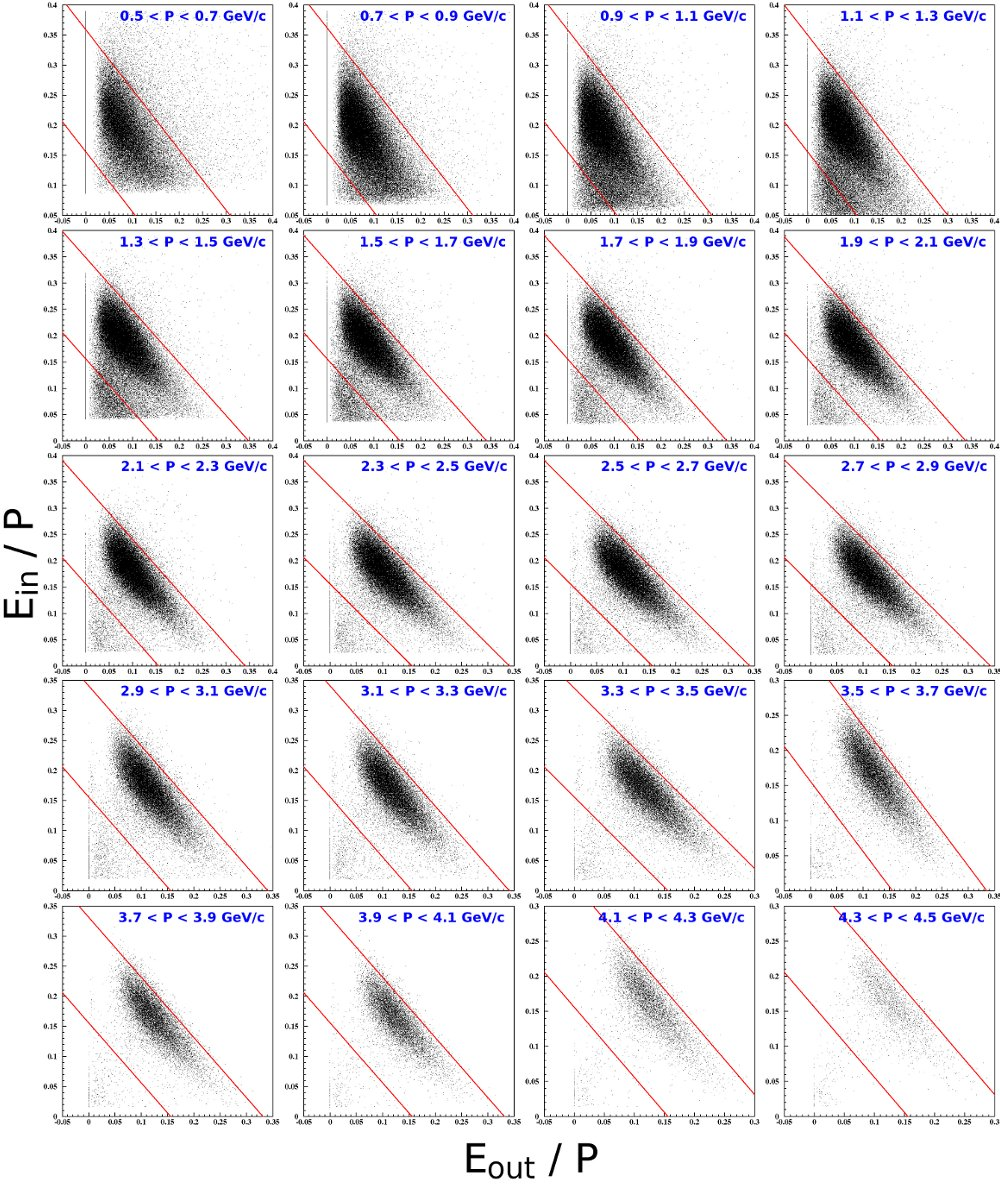
\includegraphics[width=14cm] {chap5-fig/fig02.jpg} 
\caption {Energy deposited in the inner part of the EC ($E_{in})$) as a function of the 
energy deposited in the outer part ($E_{out})$), both divided by the momentum of the 
particle. Each panel is for a different momentum range, the red lines 
illustrate the cuts from equation \ref{einout}.}
\label{eleEC}
\end{figure}

\begin{figure}[tbp]
\centering
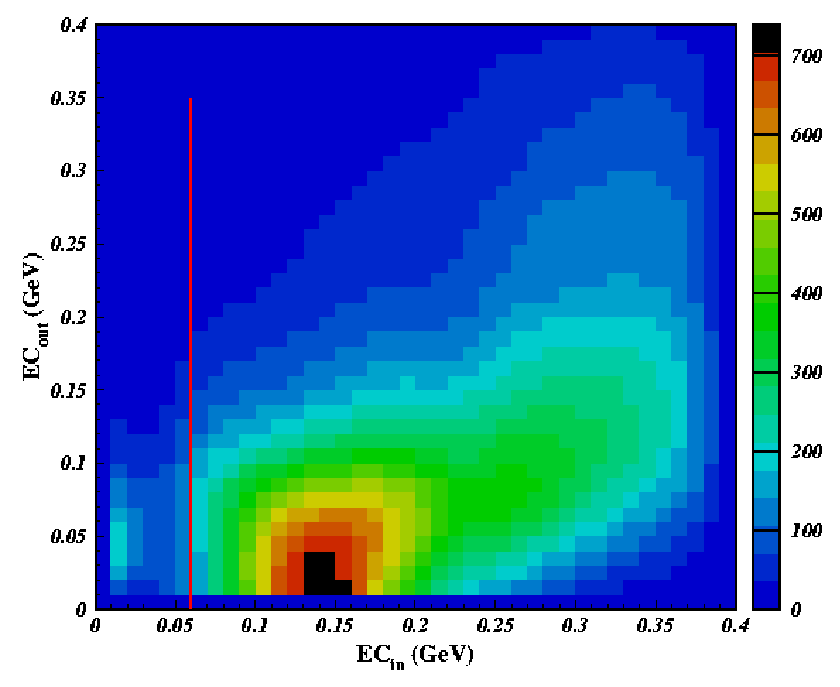
\includegraphics[width=9cm] {chap5-fig/fig03.png} 
\caption {Energy deposited in the inner part of the EC as a function of the 
energy in the outer part. The red line illustrates the cut applied for 
electron selection.}
\label{eleECi}
\end{figure}

In the CC, the mean number of photo-electrons\footnote{Photo-electrons are 
electrons produced in the front window of the Photo-Multiplier Tube (PMT) by 
single photons.} from a high energy electron is expected to be around 10.
However, hadrons can generate noise due to $\delta$ electrons produced in 
the materials of the detector. This signal is expected around 
one photo-electron, to remove it, we keep only tracks with more than 
2.5~photo-electrons (figure \ref{delta}). 

\begin{figure}[tbp]
\centering
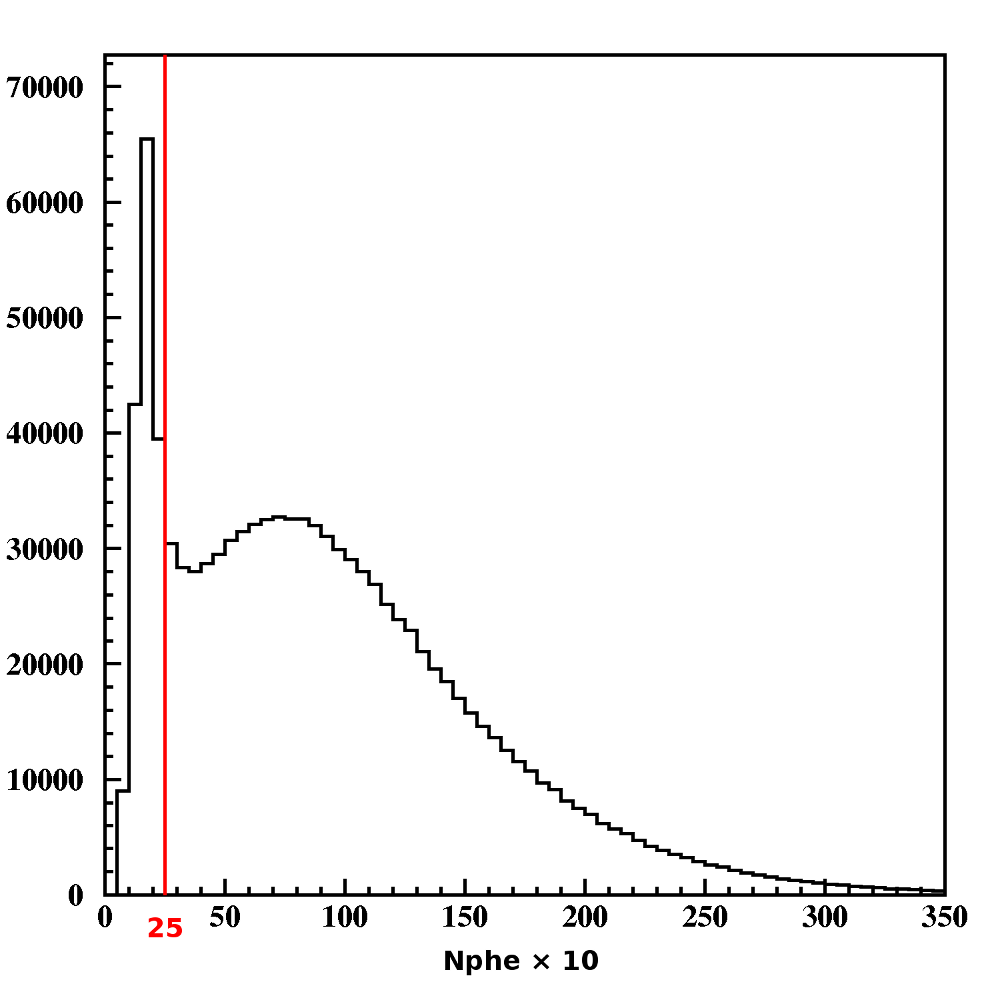
\includegraphics[width=8cm] {chap5-fig/fig04.png} 
\caption {Number of photo-electrons ($\times 10$) per tracks, the red line 
shows the cut to remove pion contamination.}
\label{delta}
\end{figure}

To select electrons, we also require that the particles are negatively charged, 
according to the bending direction of the tracks in the drift chamber.
Positively charged particles are identified as positrons. In the rest of the 
analysis we use events with only one electron and no positron to avoid any 
confusion between the scattered electron and electrons from hadronic decays or 
photon conversion to $e^+e^-$ pair, which often lead to the production of a
positron.

\subsubsection{$\pi^-$ Identification}
\label{PiId}

To identify negatively charged pions, we select negative tracks, which are not 
identified as electron. Pions are detected in the angular range from $\sim$10 to 
$\sim$140 degrees using the DC and SC only.

The identification consists mostly of a time of flight (TOF) test. We define 
$\Delta \beta = \beta_{measured} - {p \over \sqrt{p^2 + m_\pi^2}}$ and request 
$\Delta \beta$ to be zero within $\pm 0.03$. Figure \ref{PionTOF} illustrates 
the effect of this cut. We notice that there is not much negative kaons or 
anti-protons. Therefore, the contamination from these should be small (see 
section \ref{SysId} for more detailed analysis).

\begin{figure}[tbp]
\centering
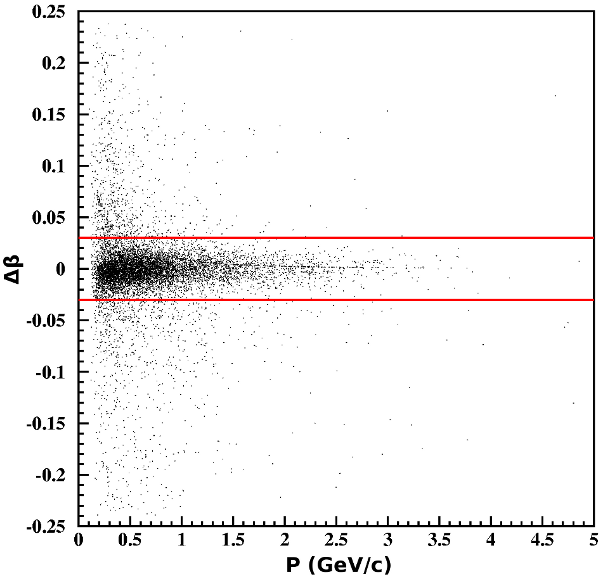
\includegraphics[width=8cm] {chap5-fig/fig05.png} 
\caption {$\Delta \beta$ as a 
function of momentum (GeV/c). Only negative particles are plotted. The red 
lines are the cuts applied to select negative pions.}
\label{PionTOF}
\end{figure}

In principle, pion identification could be improved using the Cherenkov counter 
for momentum higher than 2.5~GeV/c. But, the low efficiency observed (figure 
\ref{PionCC}), especially at momentum close to the threshold ($\sim$25\% at 
2.5~GeV/c and $\sim$50\% at 3~GeV/c), makes its use less compelling. 
Moreover, as only a very small amount of $K^-$ and no $\bar p$ are present on 
the figure \ref{PionTOF}, we decided not to use the CC for pion identification.

\begin{figure}[tbp]
\centering
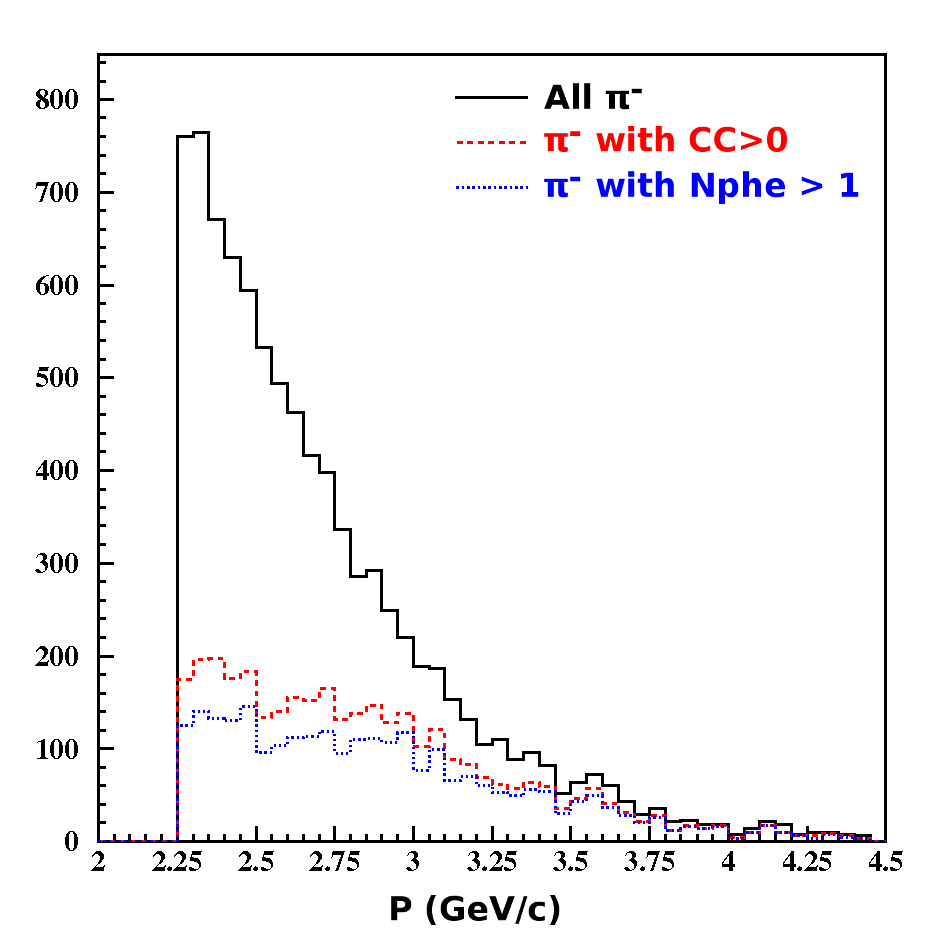
\includegraphics[width=8cm] {chap5-fig/fig06.png} 
\caption {Histograms of momentum (GeV/c) for $\pi^-$. In black are all 
identified $\pi^-$, in red pions that also fire in the Cherenkov counter and 
in blue those that fire in the Cherenkov counter with more than 
1 photo-electrons.}
\label{PionCC}
\end{figure}

\subsubsection{$\pi^+$ Identification}

The identification of positively charged pions is similar to that of negative 
pions. However, the time of flight plot is significantly more busy (figure 
\ref{PipTOF}), showing significant contamination from $K^+$ and protons at 
high momentum. As the CC is not efficient enough for hadron separation, the 
numerous kaons and protons should be removed by a tighter TOF cut:

\begin{subequations}\label{TOF-Pip}
\begin{align}
    p_\pi &\leq 3.375 \text{ GeV/c : }
  & \Delta \beta &> \max\left(-0.03,{p \over\sqrt{p^2+0.4^2}}\right), \\ 
    p_\pi &> 3.375    \text{ GeV/c : }
  & \Delta \beta &> \max\left(-0.02,{p \over\sqrt{p^2+0.7^2}}\right).
\end{align}
\end{subequations}

These cuts permit to minimize the kaon contamination, below 2.5~GeV/c, and the 
proton contamination for all momentum. The kaon contribution cannot be avoided, however 
it should remain a small contribution ($\sim$ 3\% according to simulation) 
with only a small effect on the final results (see section \ref{SysId} 
for details). Because protons could lead to even more contamination than kaons, 
a stricter cut is used at high momentum. This cut is also justified by 
HERMES data \cite{Airapetian:2007vu}, which show a very 
different behavior of the protons compared to the other hadrons (see chapter \ref{chap:data}).

\begin{figure}[tbp]
\centering
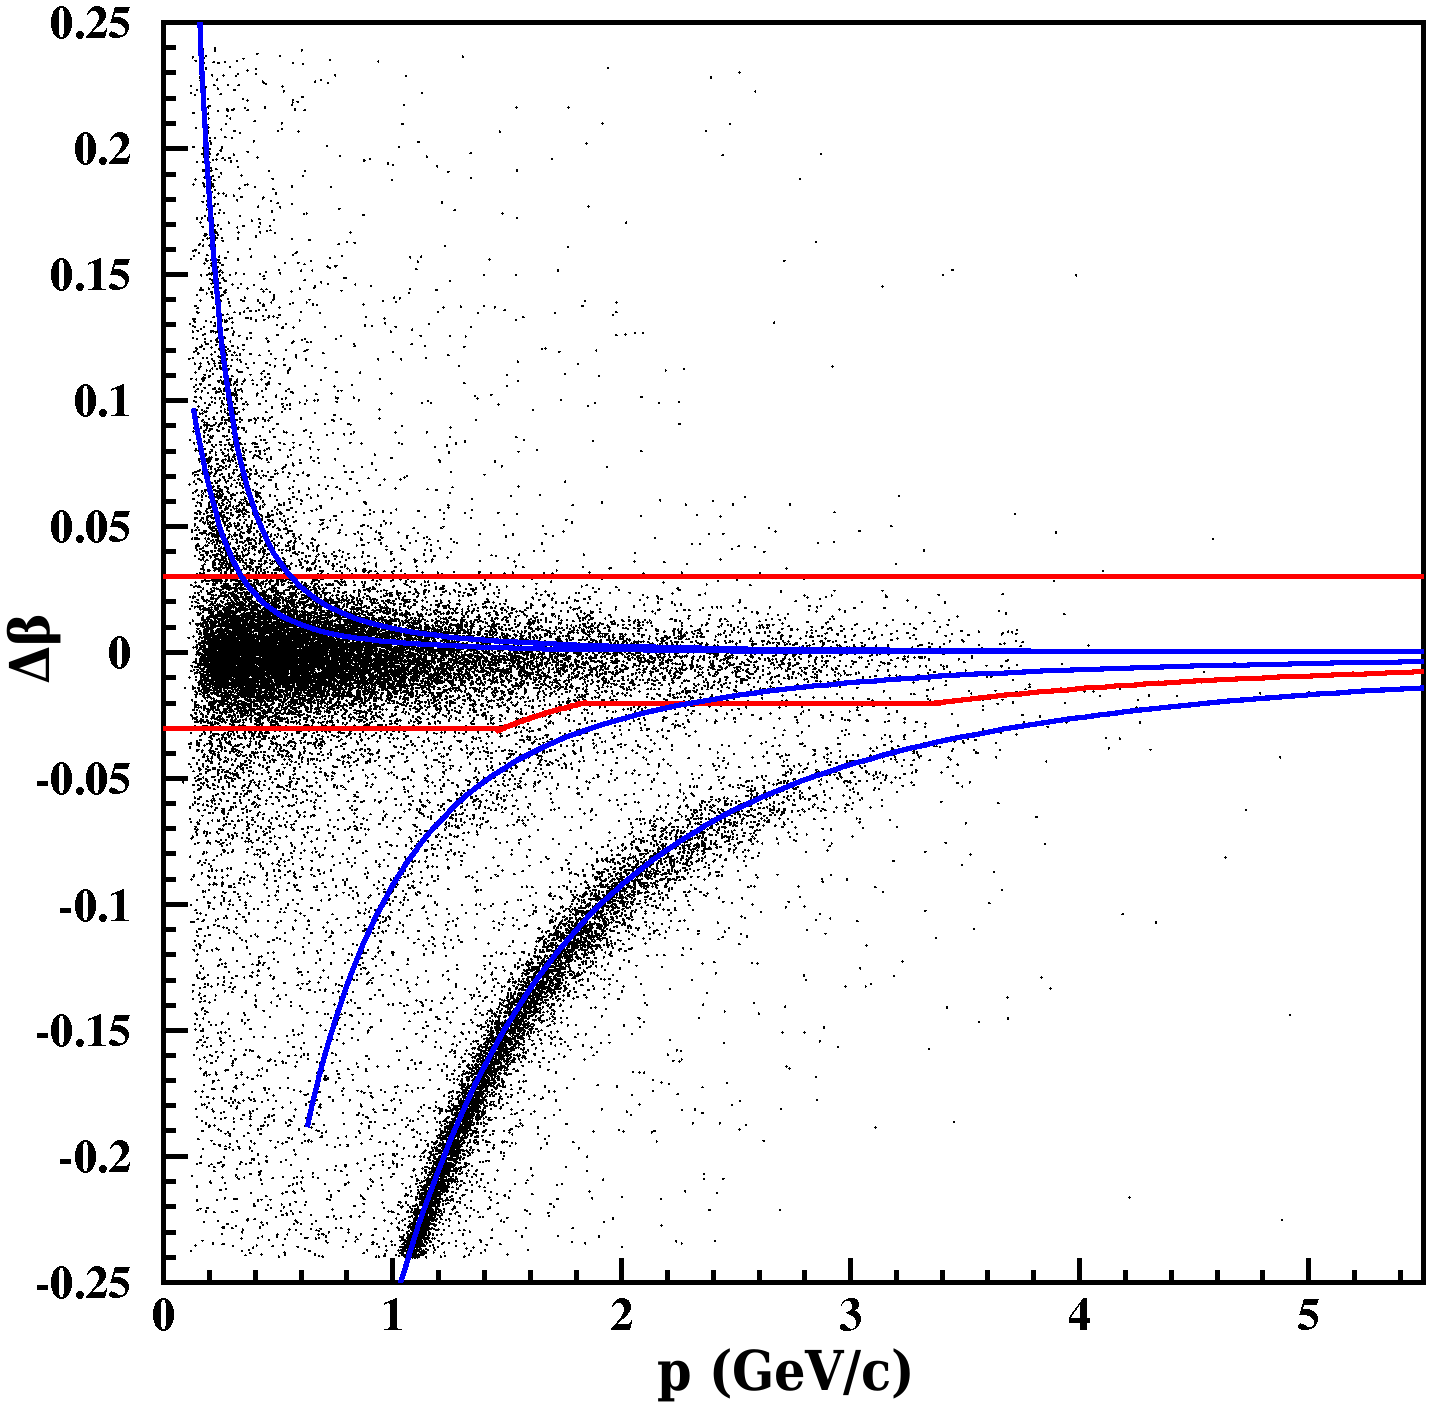
\includegraphics[width=8cm] {chap5-fig/pip_data.png} 
\caption {$\Delta \beta$ as a 
function of momentum (GeV/c). Only positive particles are shown, the red 
lines are the cuts applied to select positive pions. The blue lines indicate 
theoretical positions for other particle masses, are plotted from top to 
bottom the lines for positrons, muons, kaons and protons.}
\label{PipTOF}
\end{figure}

\subsubsection{Target Determination}

To differentiate the two targets and remove the background, we need to 
determine the origin of the particles. It appears that the different sectors 
are shifted in $z$ (figure \ref{vertex}), because of a small misalignment of 
the beam with the detector. To correct this problem, we apply the modification shown in table 
\ref{tab:vertex} for the vertex determination. Those values were determined by 
fitting the solid target position viewed by each sector.

\begin{table}[p]
  \centering
  \begin{tabular}{@{} cc @{}}
    \hline
    Sector & Shift (cm) \\ 
    \hline
    1 & + 0.1 \\ 
    2 & - 0.4 \\ 
    3 & - 0.6 \\ 
    4 & - 0.1 \\ 
    5 & + 0.4 \\ 
    6 & + 0.6 \\ 
    \hline
  \end{tabular}
  \caption{Values used to correct the vertex information for all sectors}
  \label{tab:vertex}
\end{table}

The position of the targets may also vary from one run to another, but 
this does not happen too often. Indeed, except for aluminum, the targets remain in 
the same position within one or two millimeters. The positions, in CLAS 
coordinates, are given in table \ref{tab:targets}.

\begin{table}[p]
  \centering
  \begin{tabular}{|c|c|c|c|c|c|c|}
    \hline
    Target & Carbon & Al (1) & Al (2) & Iron   & Tin    & Lead   \\ 
    \hline \hline
    Liquid & -30.1  & n/a    & n/a    & -30.2  & -30.1  & -30.1  \\ 
    Solid  & -24.7  & -25.0  & -23.8  & -24.9  & -23.8  & -24.9  \\
    \hline
  \end{tabular}
  \caption{Measured mean vertex position of targets, relative to the center of 
           CLAS (in cm). (Aluminum data are separated in two sets because the 
           target position appears to have changed at some point.)}
  \label{tab:targets}
\end{table}

\begin{figure}[p]
\centering
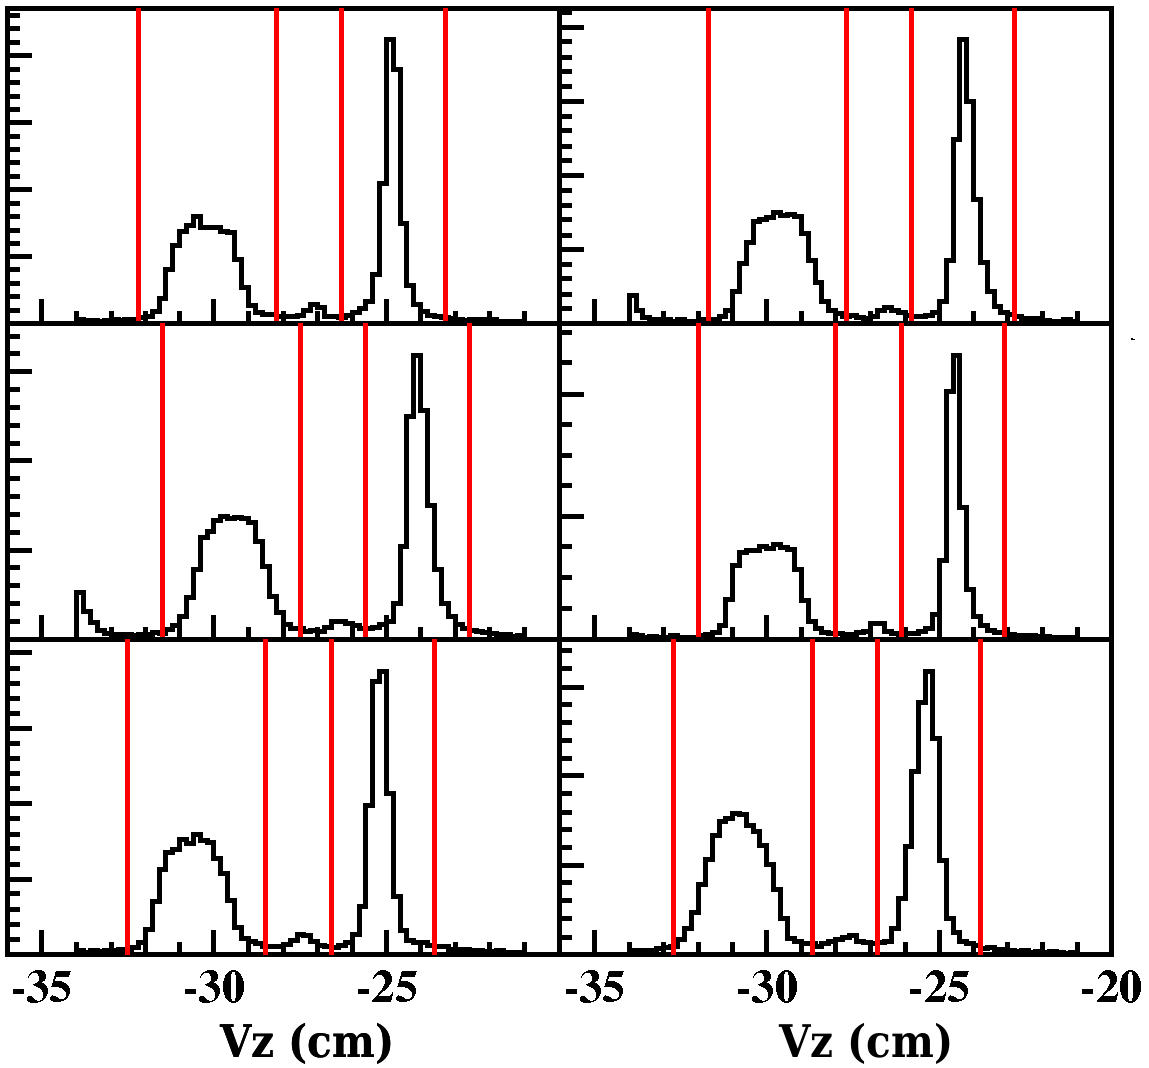
\includegraphics[width=10cm] {chap5-fig/Vertex_el_data.png}
\caption {In each sector, the reconstructed vertex of electrons along the beam
direction relatively to the center of CLAS. The red lines show the cuts 
to select the targets.}
\label{vertex}
\end{figure}

The detected electrons are associated with the solid target if their vertex 
position is at less than 1.5~cm ($\sim$3~$\sigma$) from the value of table 
\ref{tab:targets}. For the liquid target, the cut is larger, 2 cm, in order to 
account for the size of the target (see figure \ref{vertex}). The vertex of 
the pions is checked against the electron one and we request that 
$| Vz^{e^-} - Vz^{\pi} | < 3$ cm (see figure \ref{fig:dvzpi}).

\begin{figure}[tbp]
\centering
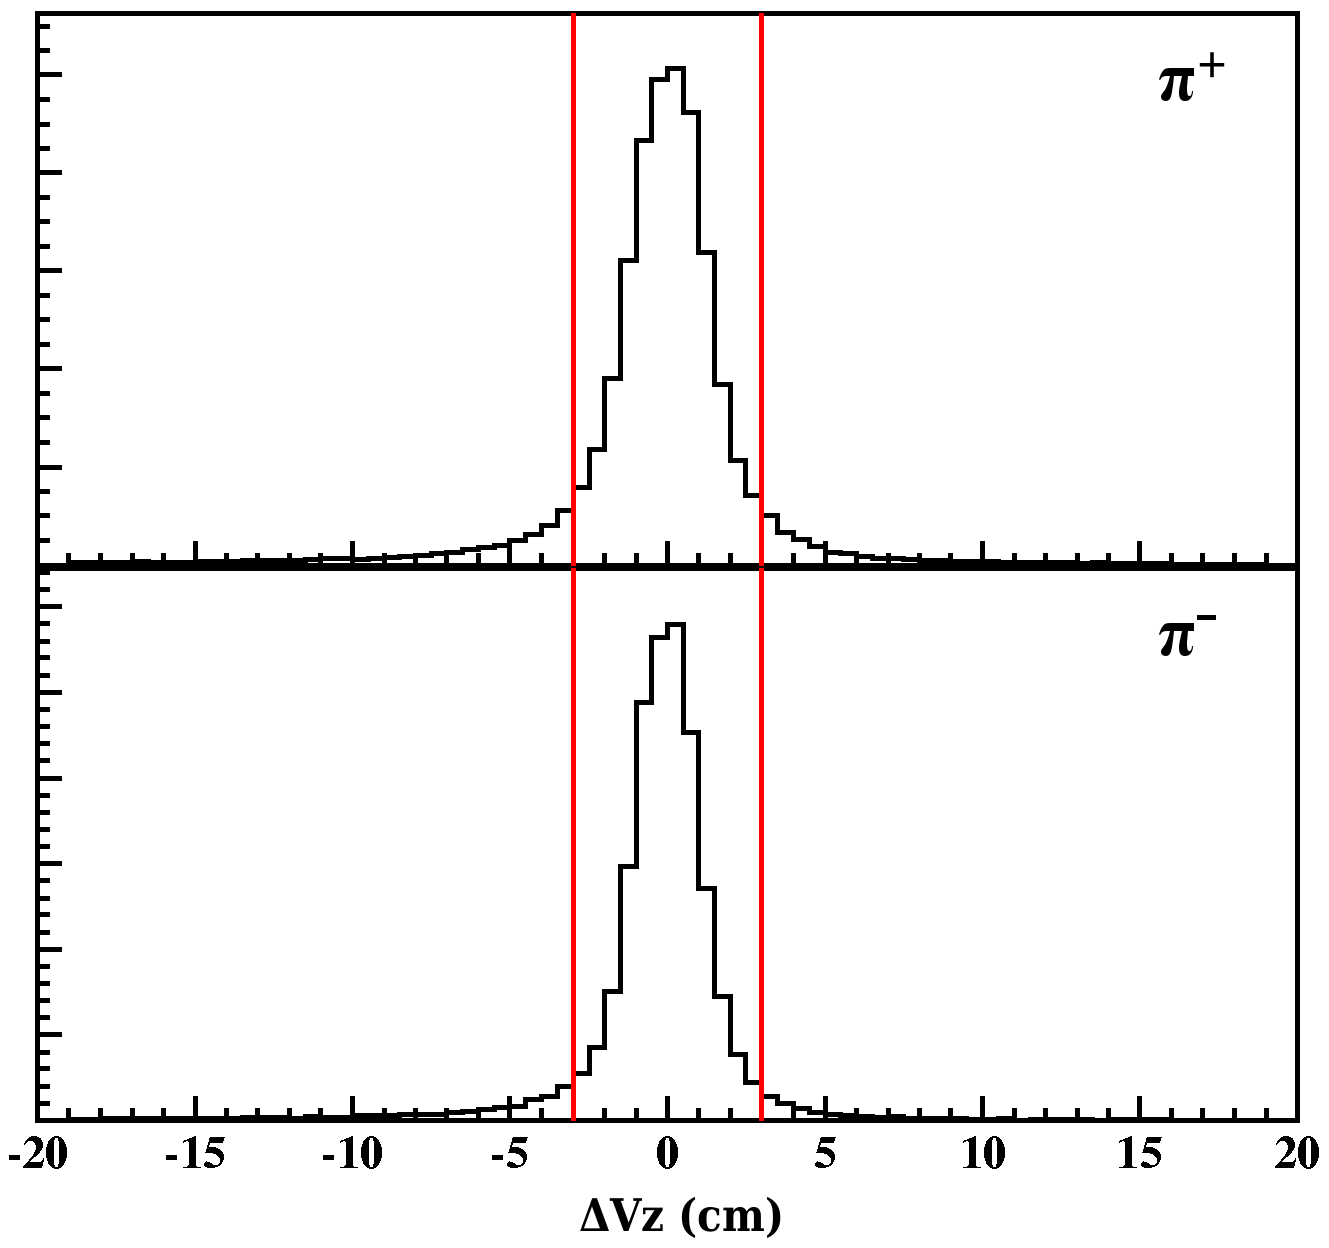
\includegraphics[width=8cm] {chap5-fig/Vertex_pi_data.png}
\caption {Distance along the beam axis between the electrons and pions 
vertexes. $\pi^+$ are plotted in the top panel and the $\pi^-$ in the bottom.
The red lines show the cuts applied to select pions.}
\label{fig:dvzpi}
\end{figure}

\subsubsection{Data Quality}

To check the quality of the runs\footnote{Runs correspond roughly to two hours
of data, they can be smaller in case of problem.}, we look at the ratio of the number of 
scattered electrons, between the liquid and solid targets. If the beam is 
hitting other materials than the targets or if the detector is not working 
properly this ratio can be off and indicates a problematic run. The figure 
\ref{DataQ} shows the values obtained; we fit the 
mean value for all runs of each target and eliminate runs away by more than 
5$\sigma$. We note that the ratios are coherent with target thicknesses given 
in \cite{Hakobyan:2008zz} except for carbon. Because of this, the density of 
the carbon target was remeasured recently and found to be coherent with the 
data\footnote{i.e. (1.747+/-0.0007)g/cm$^3$ instead of 2.235 g/cm$^3$}.

\begin{figure}[tbp]
\centering
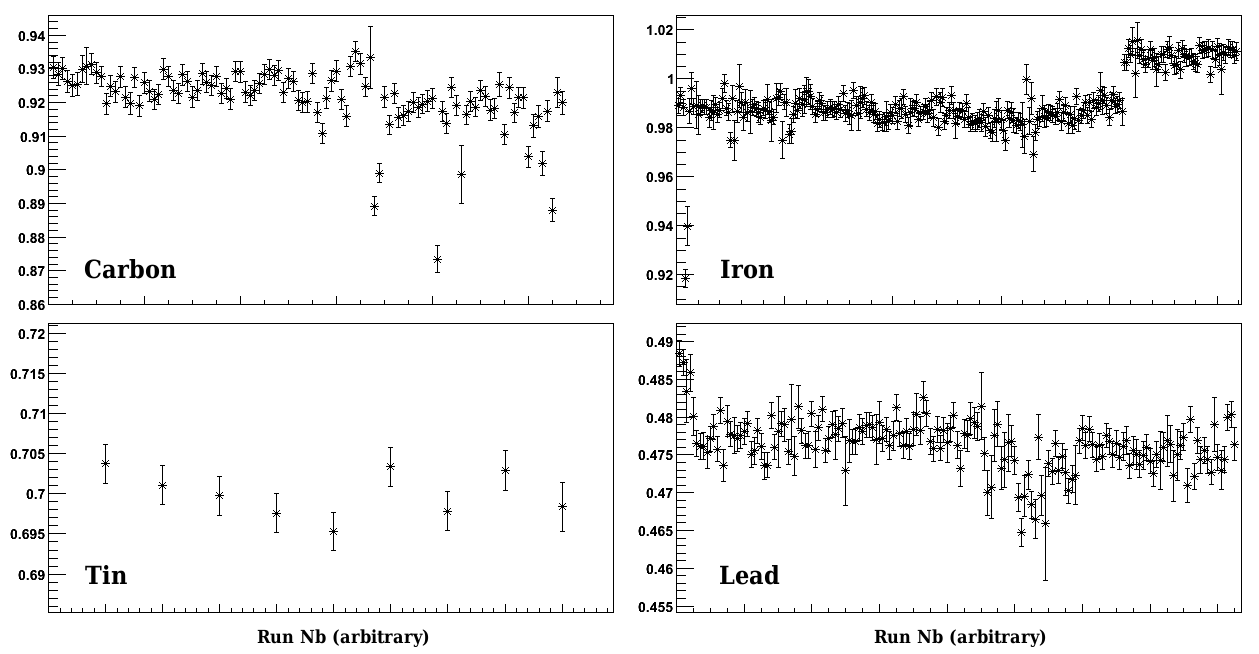
\includegraphics[width=15cm] {chap5-fig/TargetElRatio.png}
\caption {Ratio of the number of electrons scattered by the targets (solid over deuterium) 
for each run.}
\label{DataQ}
\end{figure}

\subsection{Extraction of Multiplicity Ratio and $\Delta$P$_\perp^2$}
\label{sec:obs}

Since we are interested in deep inelastic scattering, we use the following 
cuts: $Q^2 > 1$~GeV$^2$/c$^2$ and $W > 2$~GeV. We also apply a cut $y < 0.85$ to 
reduce the impact of radiative effects, which will be discussed in more details in 
the section \ref{RadCor}.

\subsubsection{Method}
\label{RatioCalc}

Once the identification is done, the calculation of the observables is 
straight forward and the statistical errors are calculated with this expression

\begin{equation}
{\delta \left ( R_A^h \right ) \over R_A^h} = \sqrt{ 1 /N_A^h + 1/ N_A^e +1/N_D^h + 1/N_D^e}
\end{equation}
and
\begin{equation}
\left ( \delta \left ( \Delta \langle P_\perp^2 \rangle \right ) \right )^2 = 
   \left ({\langle P_\perp^4 \rangle - \langle P_\perp^2 \rangle ^2}\right )_A / N_A^h
 + \left ({\langle P_\perp^4 \rangle - \langle P_\perp^2 \rangle ^2}\right )_D / N_D^h.
\end{equation}

The implementation of acceptance and radiative corrections is done through weights
given to each particles depending on its kinematic. The multiplicity ratio becomes

\begin{equation}
R_A^h (Q^2,\nu,z_h,P_\perp^2) = {{\sum \omega_A^h (Q^2,\nu,z_h,P_\perp^2) / \sum \omega_A^e (Q^2,\nu)} 
                       \over {\sum \omega_D^h (Q^2,\nu,z_h,P_\perp^2) / \sum \omega_D^e (Q^2,\nu)}},
\end{equation}
with $\omega$ the weights and all the sums running over all measured particles.
The expression for the transverse momentum broadening remains
\begin{equation}
\Delta \langle P_\perp^2 \rangle = \langle P_\perp^2 \rangle_A - \langle P_\perp^2 \rangle_D,
\end{equation}
but with
\begin{equation}
\langle P_\perp^2 \rangle = {\sum P_\perp^2 \times \omega (Q^2,\nu,z_h,P_\perp^2) \over \sum \omega (Q^2,\nu,z_h,P_\perp^2)}.
\end{equation}

This expressions leads to new expressions for the statistical error uncertainties: 

\begin{equation}
{\delta \left ( R_A^h \right ) \over R_A^h} = 
      \sqrt{ \left ( {\sum {\omega^h_A}^2 \over \left (\sum \omega^h_A \right )^2} \right ) 
           + \left ( {\sum {\omega^e_A}^2 \over \left (\sum \omega^e_A \right )^2} \right ) 
           + \left ( {\sum {\omega^h_D}^2 \over \left (\sum \omega^h_D \right )^2} \right ) 
           + \left ( {\sum {\omega^e_D}^2 \over \left (\sum \omega^e_D \right )^2} \right ) }
\end{equation}
 and 
\begin{equation}
\begin{split}
\left ( \delta \left ( \Delta \langle P_\perp^2 \rangle \right ) \right )^2 = 
   \left ({{\sum \omega^h_A P_\perp^4 }\over{\sum \omega^h_A}} - \left ({\sum \omega^h_A P_\perp^2 }\over{\sum \omega^h_A}\right )^2 \right ) 
         \times \left ( {\sum \left ( {\omega^h_A}^2 \right ) \over \left ( \sum \omega^h_A \right ) ^2 }\right ) \\
 + \left ({{\sum \omega^h_D P_\perp^4 }\over{\sum \omega^h_D}} - \left ({\sum \omega^h_D P_\perp^2 }\over{\sum \omega^h_D}\right )^2 \right ) 
	 \times \left ( {\sum \left ( {\omega^h_D}^2 \right ) \over \left ( \sum \omega^h_D \right ) ^2 }\right ).
\end{split}
\end{equation}

\subsubsection{Preliminary Results}
\label{prelim}

We present in figure \ref{fig:prelim} few preliminary results, before the application of any correction, with the goal to 
provide a first idea on data quality. The preliminary results will also be used to 
illustrate the effects of the corrections discussed below.

\begin{figure}[htb]
\centering
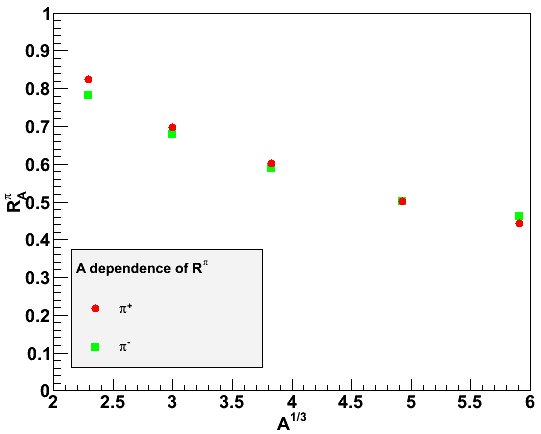
\includegraphics[width=7.4cm] {chap5-fig/a_RvA.png} 
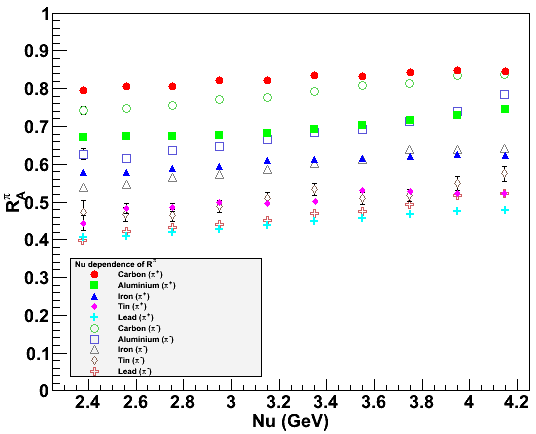
\includegraphics[width=7.4cm] {chap5-fig/a_RvZ.png} 
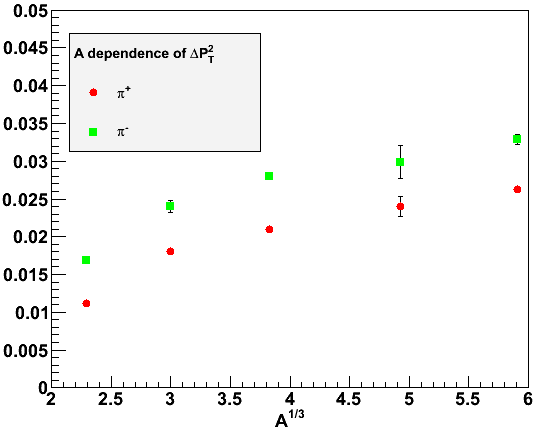
\includegraphics[width=7.4cm] {chap5-fig/a_PvA.png} 
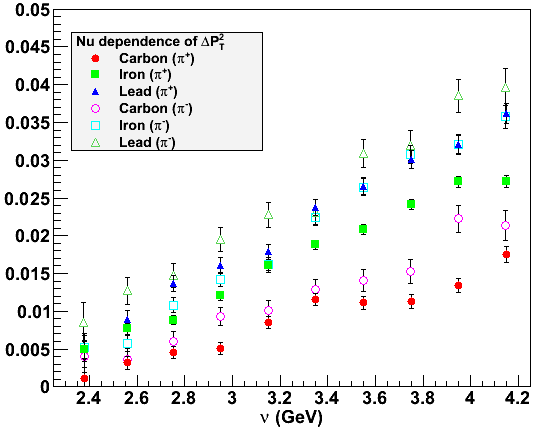
\includegraphics[width=7.4cm] {chap5-fig/a_PvNu.png} 
\caption {Results for multiplicity ratios (top) and transverse momentum 
broadening (bottom) without correction.}
\label{fig:prelim}
\end{figure}


\subsection{Corrections}
\label{sec:corrections}

\subsubsection{Acceptance Correction}
\label{sec:accept}

The acceptance correction consists of applying weights to the events in 
experimental data to correct for the inefficient parts of the detectors.
Incidentally, it also corrects for small other issues of detection,
such as misidentification and scattering on detectors materials. The quality 
of the correction depends on the ability of the simulation to reproduce the 
experiment, the statistics accumulated and the size of interfering effects, such 
as bin migration.

\paragraph{Simulation}
\label{sec:simul}

To correct for acceptance effects, we simulated a total of a 100 million events 
per target ($^2$H, C, Fe and Pb) using the PYTHIA \cite{Sjostrand:2006za} 
event generator slightly modified to include Fermi motion effects. The 
generated events are processed by the CLAS software (GSIM, GPP and user\_ana) 
to simulate the detector and the reconstruction process similarly to the one for experimental data.

Then the simulated data are processed in a similar way than the experimental data by 
applying the cuts described in the section \ref{sec:pid}. Overall the 
simulation reproduces quite well the detectors responses, yet two issues might 
affect us and have to be understood. First, the efficiency of the CC is overestimated in the simulation. 
On the electron side the signal is a little stronger in the simulation (11 
photo-electrons) compared to experimental data (8 photo-electrons), but this 
feature should not affect us too much, because we are cutting only the tail of the 
distribution in both cases. For pion identification, as mentioned in section \ref{PiId},
we do not use the CC because of its unexpectedly low efficiency 
We observe, in the simulation, a much better detector response than in experiment 
(figure \ref{simPionCC} compared to figure \ref{PionCC}), this result also advocates against the use of the CC in the 
particle identification. Indeed, the poor reproduction of the experimental signal would introduce a bias in our acceptance correction. 
Second, in figure \ref{vertex} the cuts on vertex are shifted from one sector 
to another, since the simulation have perfect alignment of beam with CLAS this 
feature is not present in the simulated data. Therefore, we do not apply the 
shift from the table \ref{tab:vertex} to the simulation; results are shown in 
figure~\ref{simvertex}.

\begin{figure}[tpb]
\centering
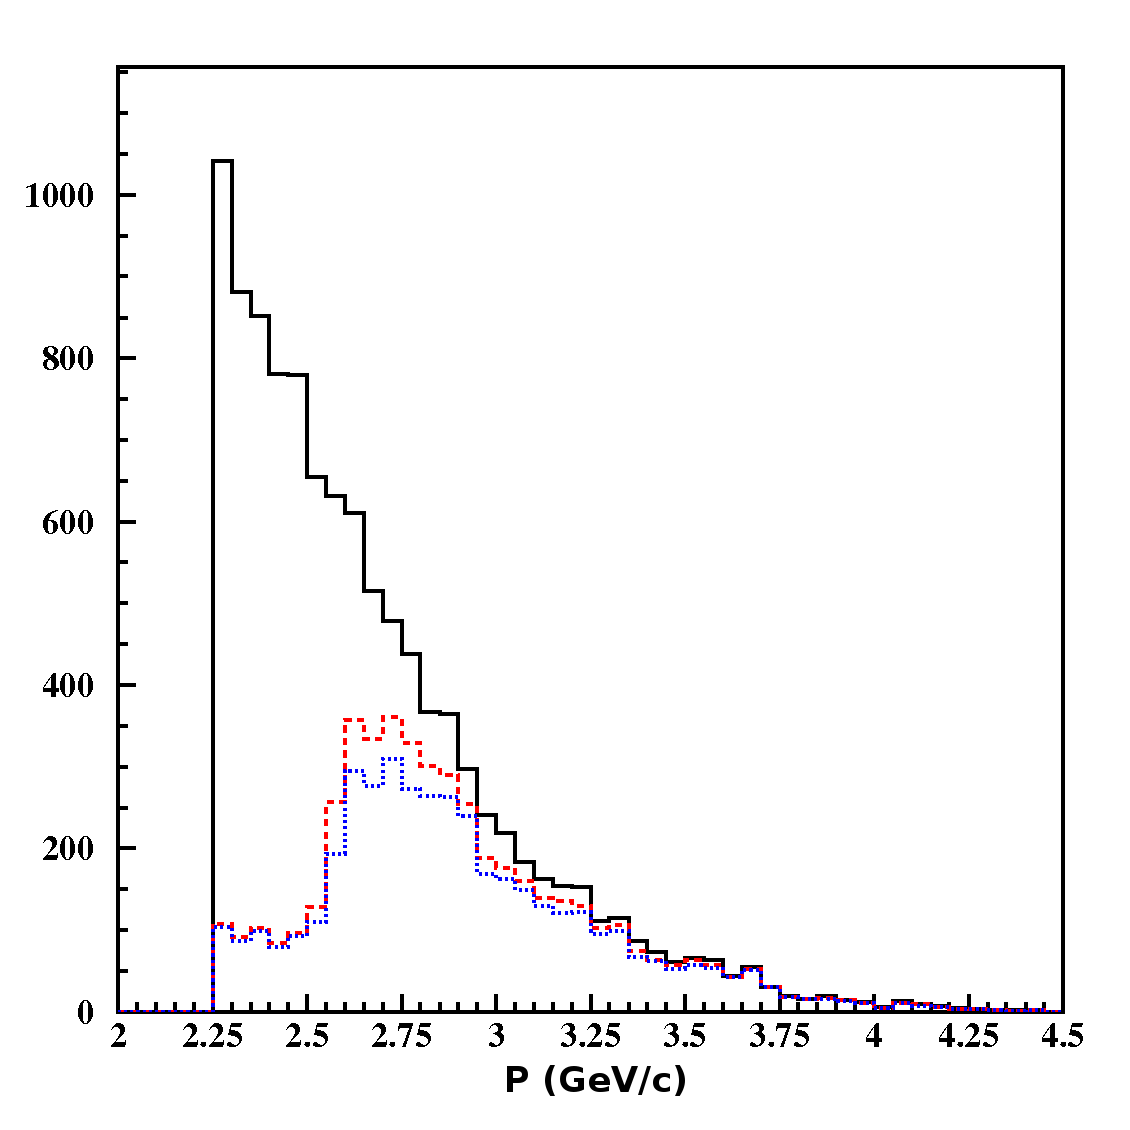
\includegraphics[width=9cm] {chap5-fig/fig06simul.png} 
\caption {Histograms of momentum (GeV/c) of $\pi^-$ for {\bf simulated data}.
In black are all identified $\pi^-$, in red pions that also fire in the 
Cherenkov counter and in blue those that fire in the Cherenkov counter with 
more than one photo-electron.}
\label{simPionCC}
\end{figure}

\begin{figure}[tpb]
\centering
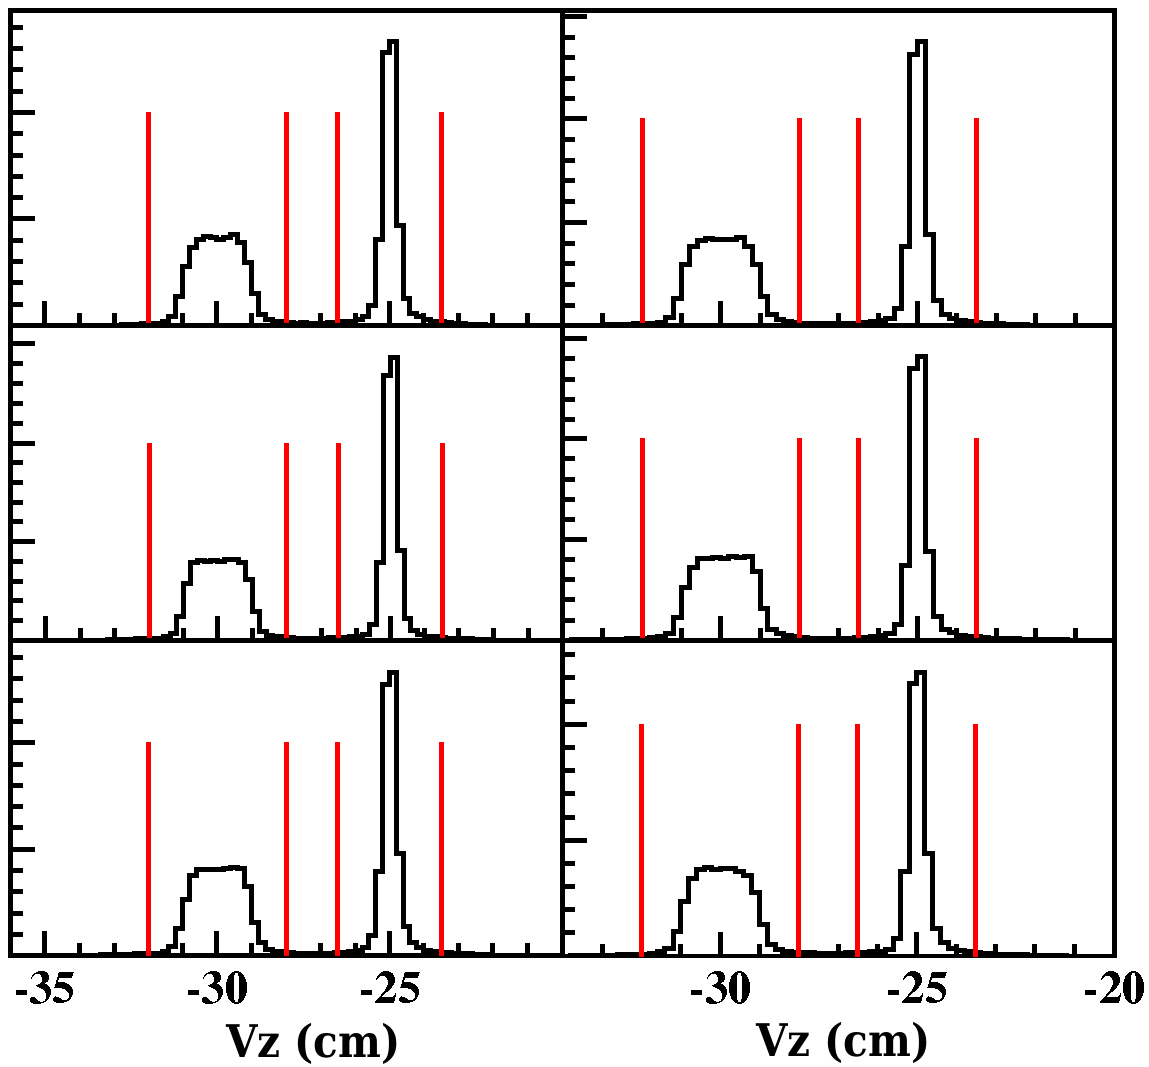
\includegraphics[width=9cm] {chap5-fig/Vertex_el_sim.png}
\caption {Reconstructed vertex position, along the beam direction, with values 
relative to CLAS center, for electrons from {\bf simulated data} and each 
sector. The red lines show the cuts used to select the targets.}
\label{simvertex}
\end{figure}

The kinematic distributions from the simulation are compared to the 
experimental ones. This is important for the acceptance correction, to see 
whether or not, we can integrate over these variables for the correction.
Comparisons between simulation and experiment are shown in figures 
\ref{fig:compNuQ2} to \ref{fig:compPhih}. The agreement is reasonable, but not 
perfect. The differences are due to the PYTHIA simulation, which is not including some 
physical effects, such as radiative and diffractive processes.

\begin{figure}[tbp]
\centering
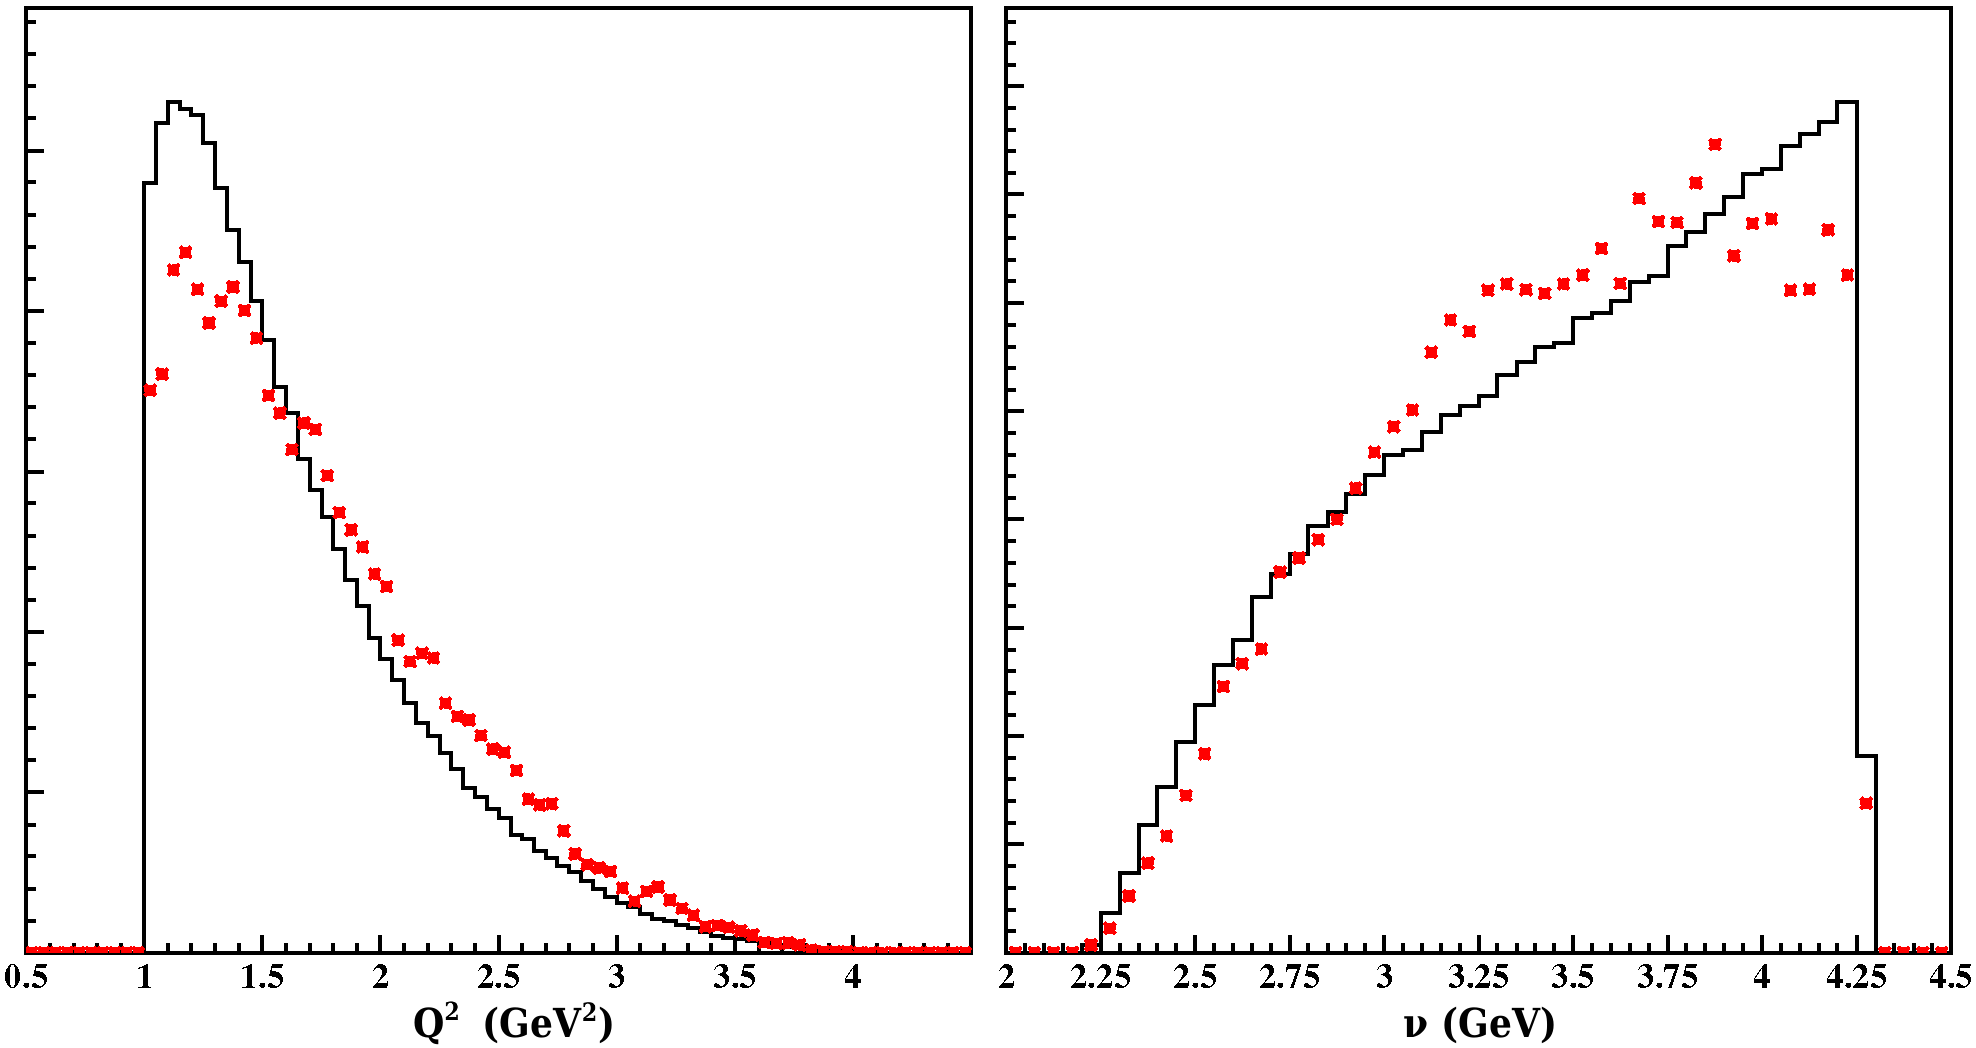
\includegraphics[width=12cm] {chap5-fig/El_compar.png}
\caption {Comparisons, for $Q^2$ (GeV$^2$/c$^2$) and $\nu$ (GeV), of the distributions
from simulated (red crosses) and experimental (histogram) data using deuterium target.}
\label{fig:compNuQ2}
\end{figure}

\begin{figure}[tbp]
\centering
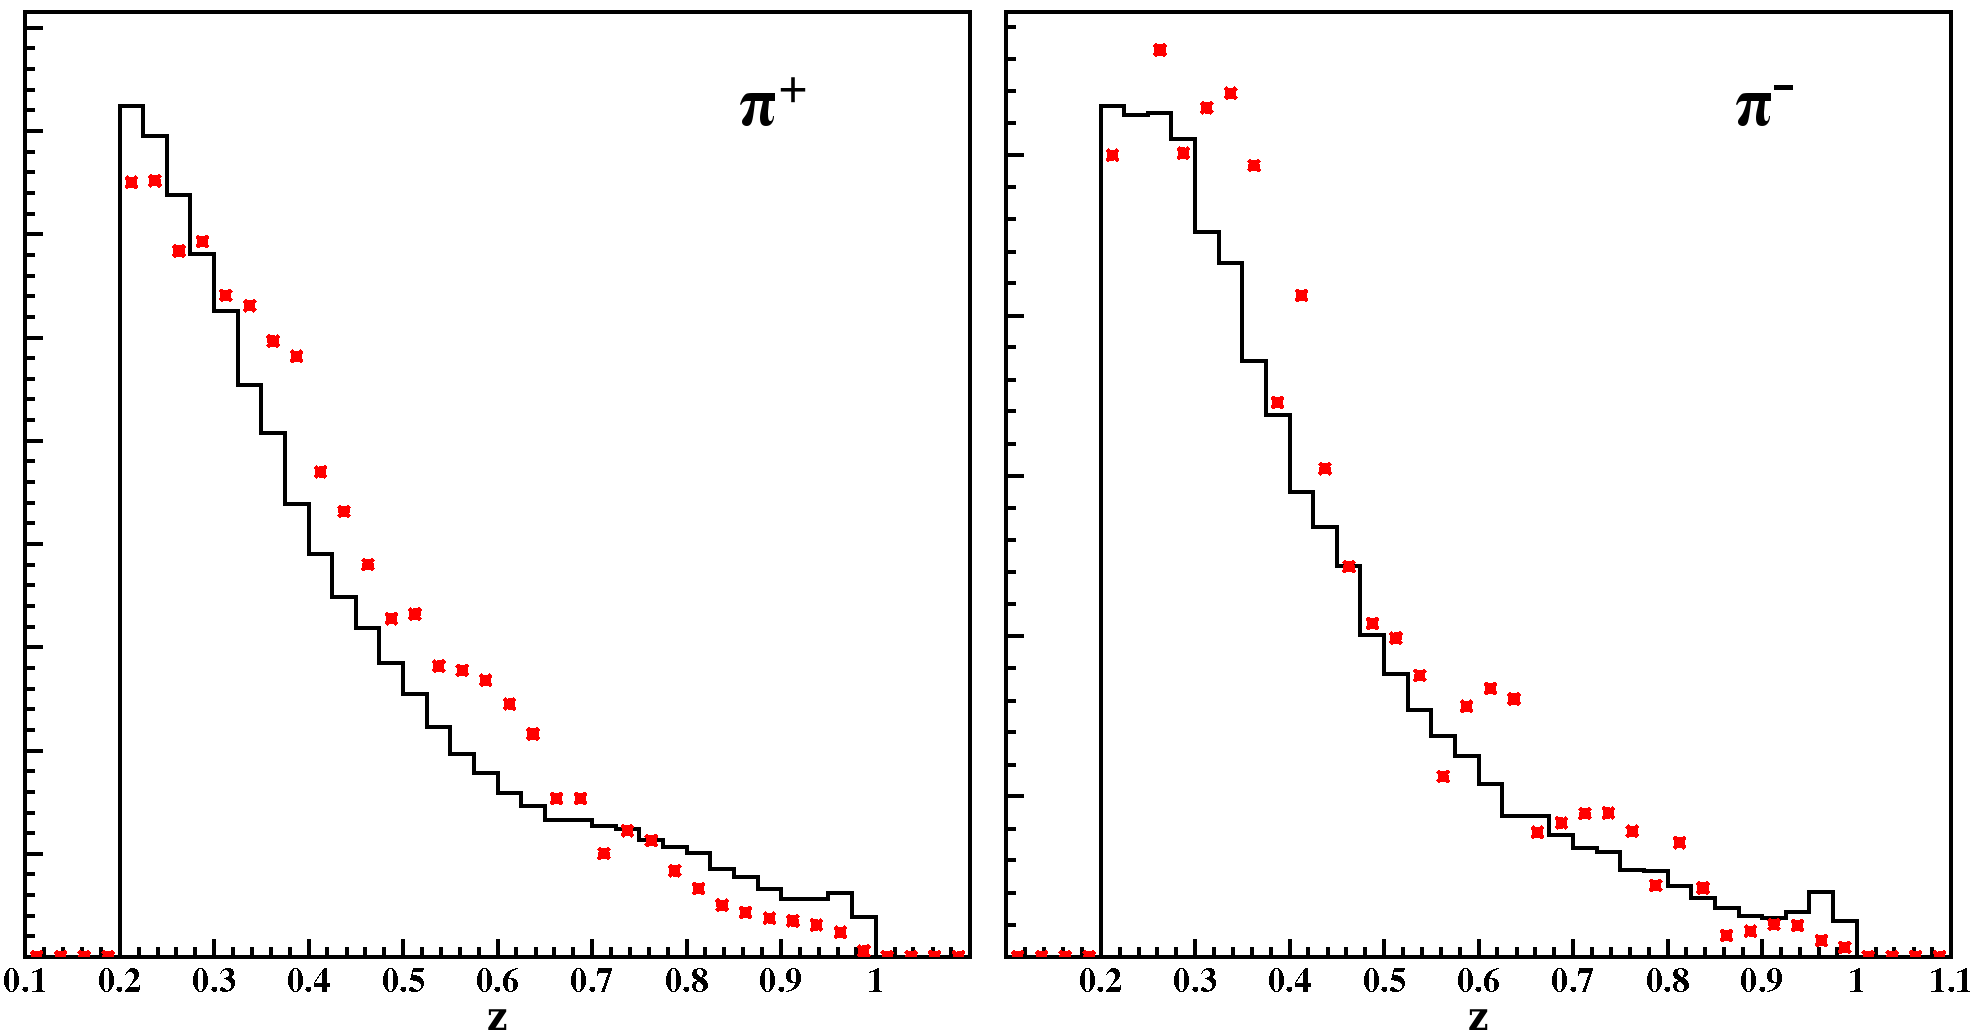
\includegraphics[width=12cm] {chap5-fig/z_compar.png}
\caption {Comparisons, for $z$ of charged pions, of the distributions
from simulated (red crosses) and experimental (histogram) data using deuterium target.}
\label{fig:compZ}
\end{figure}

\begin{figure}[tbp]
\centering
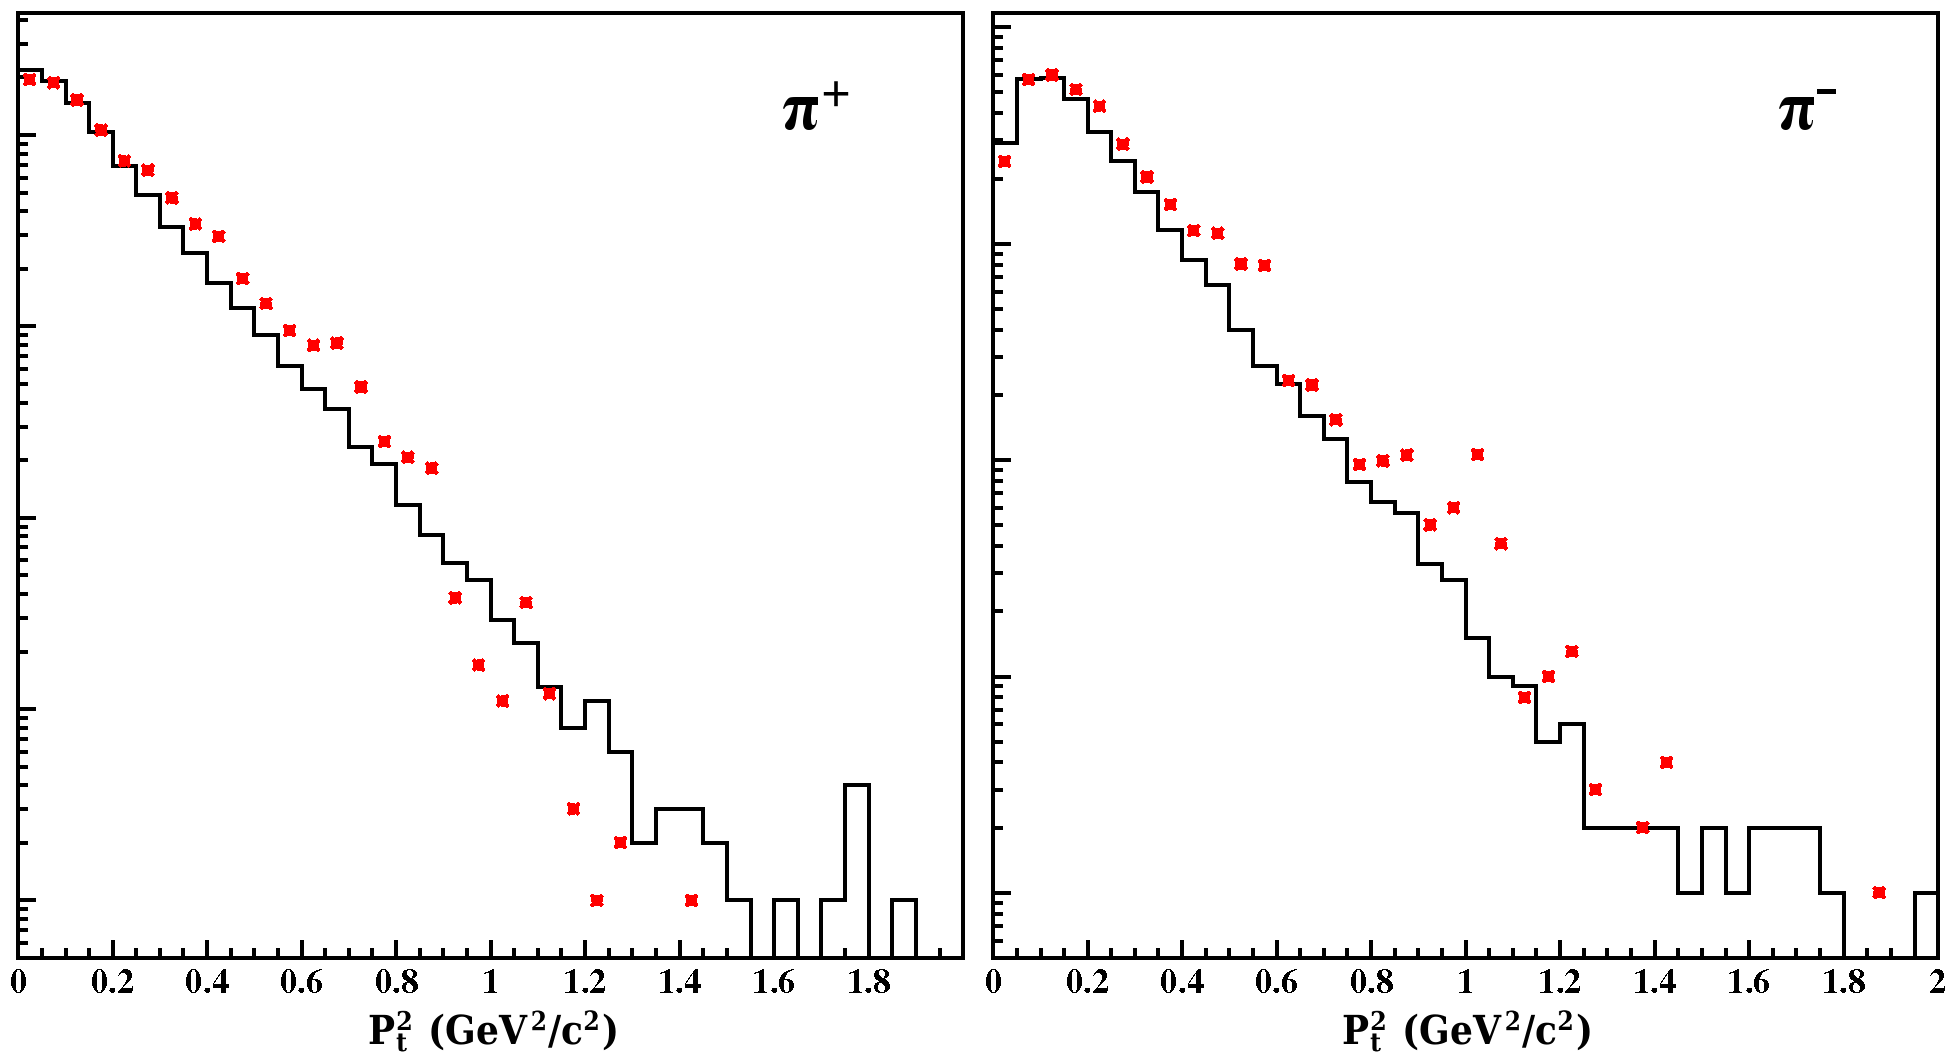
\includegraphics[width=12cm] {chap5-fig/pts_compar.png}
\caption {Comparisons, for \pt (GeV$^2$/c$^2$) of charged pions, of the distributions
from simulated (red crosses) and experimental (histogram) data using deuterium target.}
\label{fig:compPts}
\end{figure}

\begin{figure}[tbp]
\centering
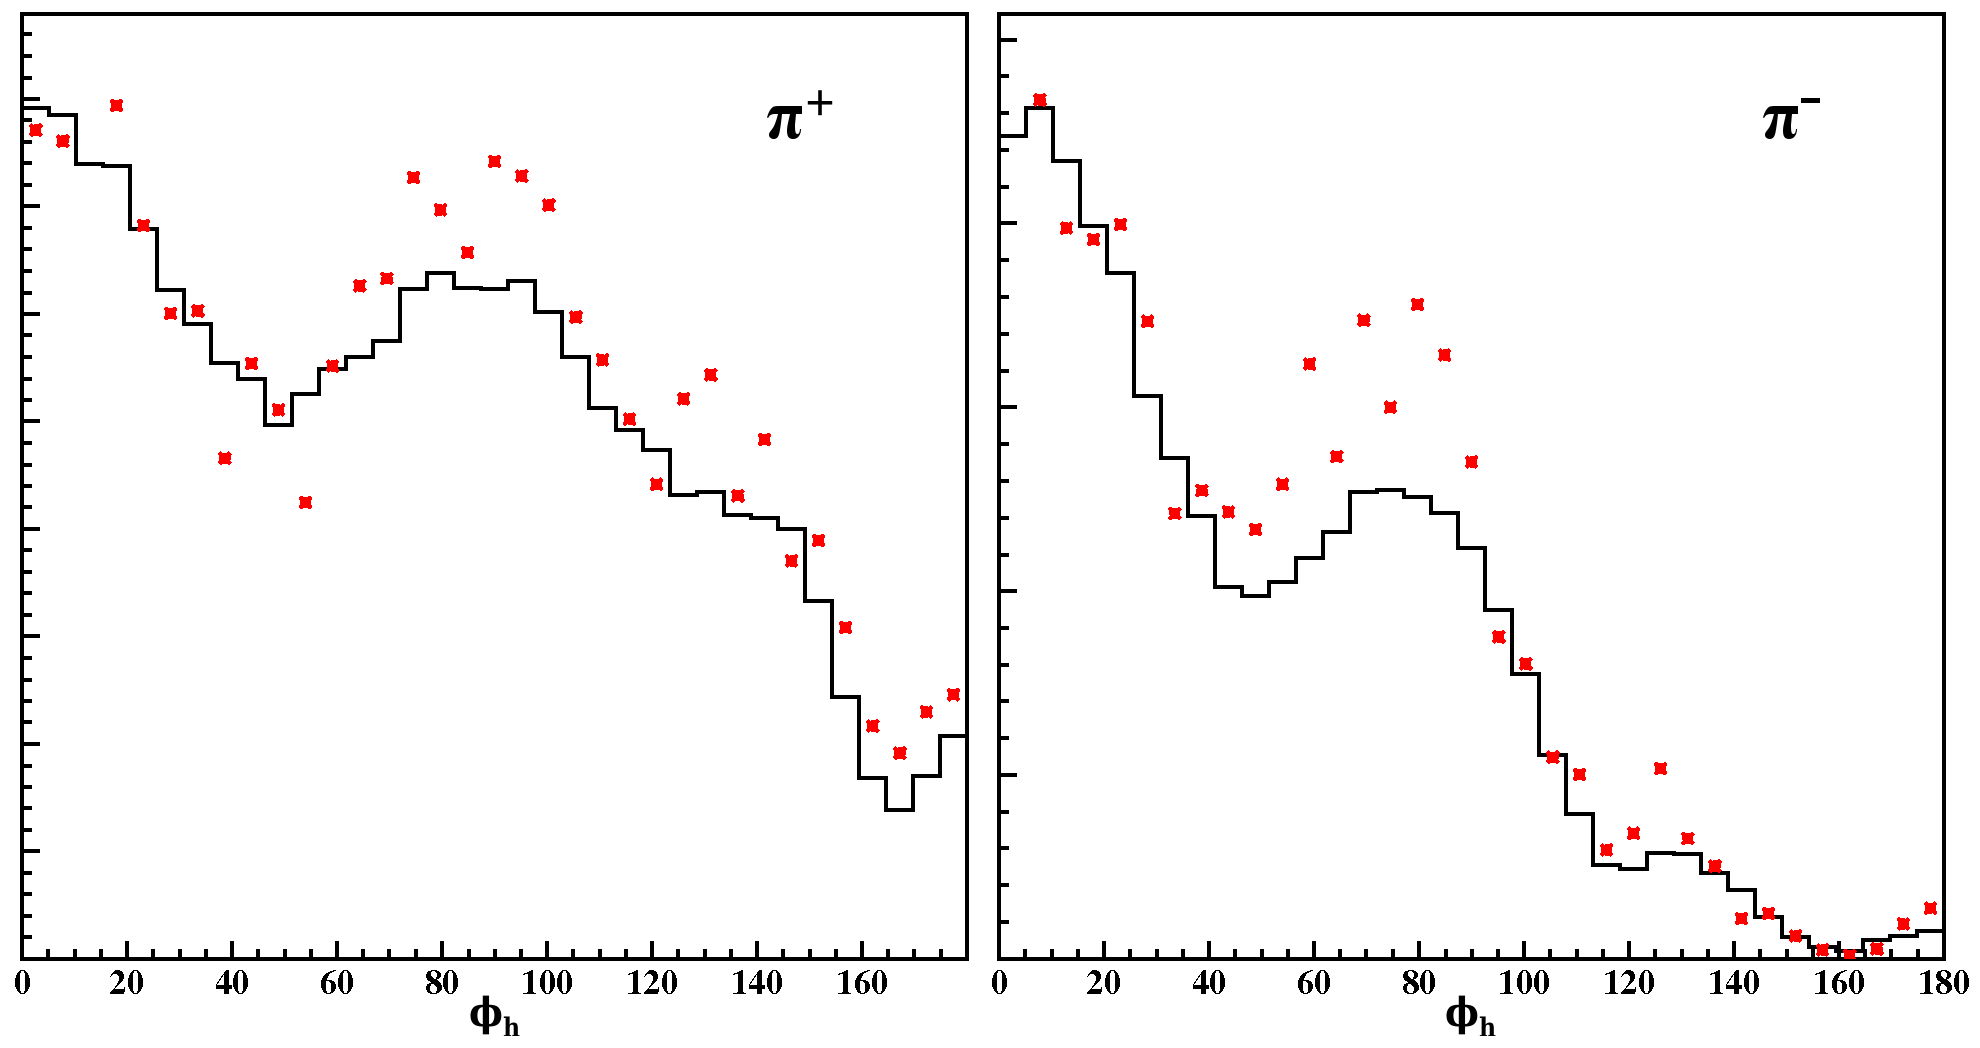
\includegraphics[width=12cm] {chap5-fig/phih_compar.png}
\caption {Comparisons, for $\phi_h$ of charged pions, of the distributions
from simulated (red crosses) and experimental (histogram) data using deuterium target.}
\label{fig:compPhih}
\end{figure}


\paragraph{Correction of the Data}

The acceptance is defined as the ratio of reconstructed events over generated ones,

\begin{equation}
\label{eq:acc}
\text{Acc} = {N_{rec} \over N_{gen}}.
\end{equation}

The data is corrected using weights defined as $\omega = 1/\text{Acc}$. The 
$\omega$ coefficient are calculated in many bins, in order to be independent of 
the imperfections of the event generator. However, an excess of bin could results into a strong 
bin migration\footnote{Fraction of events not reconstructed in the bin they 
were produced in.}, which might introduce a bias if it becomes a large effect.

We use a 4-dimensional binning to divide the large phase space available to 
the two particles in the measured final state. To evaluate the systematic error 
associated to the correction, we use two different binning, which are 
presented in the table \ref{tab:AcceptBinning}. The total number of bins is 
constrained by the amount of data generated and has to be maintained 
reasonably low in order to keep a good statistical precision and reasonable 
bin migration.

\begin{table}[htbp]
  \centering
  \begin{tabular}{@{} cc @{}}
    \hline
    Variable & Number of bins \\ 
    \hline
    $\nu$    & 5 \\
    $x_{Bj}$ & 5 \\
    $p_h$    & 7 \\
    $t$      & 7 \\
    \hline
    Total    & 1225 \\
    \hline
  \end{tabular}
  \begin{tabular}{@{} c @{}}
  ~~~~~~\\
  ~~~~~~\\
  \end{tabular}
  \begin{tabular}{@{} cc @{}}
    \hline
    Variable & Number of bins \\ 
    \hline
    $Q^2$    & 5 \\
    $\nu$    & 5 \\
    $z_h$    & 7 \\
    $t$      & 7 \\
    \hline
    Total    & 1225 \\
    \hline
  \end{tabular}
  \caption{Variables and their associated number of bins used for the 
   multi-dimensional binning of the acceptance correction. The left panel 
   shows the variables used for the correction and the right panel the 
   variables used for the evaluation of the systematic error.}
  \label{tab:AcceptBinning}
\end{table}

The weights ($\omega_{\pi^\pm}(\nu,x_{Bj},p_h,t)$) are then extracted from 
the simulation using equation \ref{eq:acc}, however, it appears that these should not be used directly.
Three factors are sources of problematic bins:
\begin{itemize}
 \item too large weight values, i.e. very small acceptance;
 \item very few events reconstructed, leading to large statistical errors;
 \item many events that were generated in another bin (bin migration).
\end{itemize}
To remove these bins we apply the following cuts:
\begin{equation} \label{eq:AccL1}
\left ({\delta \omega \over \omega}\right ) ^2 \times {R_c \over \omega} < 2,
\end{equation}
and
\begin{equation} \label{eq:AccL2}
N_{rec} > 4,
\end{equation}
with $\delta \omega / \omega$ the relative error on the weight and $R_c$ the 
proportion of events in the bin initially generated in another bin. Figure 
\ref{fig:AccCoef} shows the distributions of $\omega$, after the cuts. Around 
900 bins remain for both targets, but we notice that weights are much larger 
for $\pi^-$, indicating a larger correction, compared to $\pi^+$. In order to 
maximize the acceptance and reduce the sensitivity to the cuts applied on the 
weights, which are arbitrary, the bin weights are corrected. We apply a 
reweighting by calculating a new acceptance in a two dimensional binning:
\begin{equation}
\text{Acc}_2(\nu,p_h) = {\sum_{rec} \omega (\nu,x_{Bj},p_h,t)\over N_{gen}(\nu,p_h)}.
\end{equation}
with $\omega$ either the previously calculated weights or one for the 
excluded bins.
One of the criteria for setting the limits in equation \ref{eq:AccL1} and 
\ref{eq:AccL2} is to keep the reweighting factors $\omega_2 = 1/\text{Acc}_2$ at a few 
percents level.

\begin{figure}[tbp]
\centering
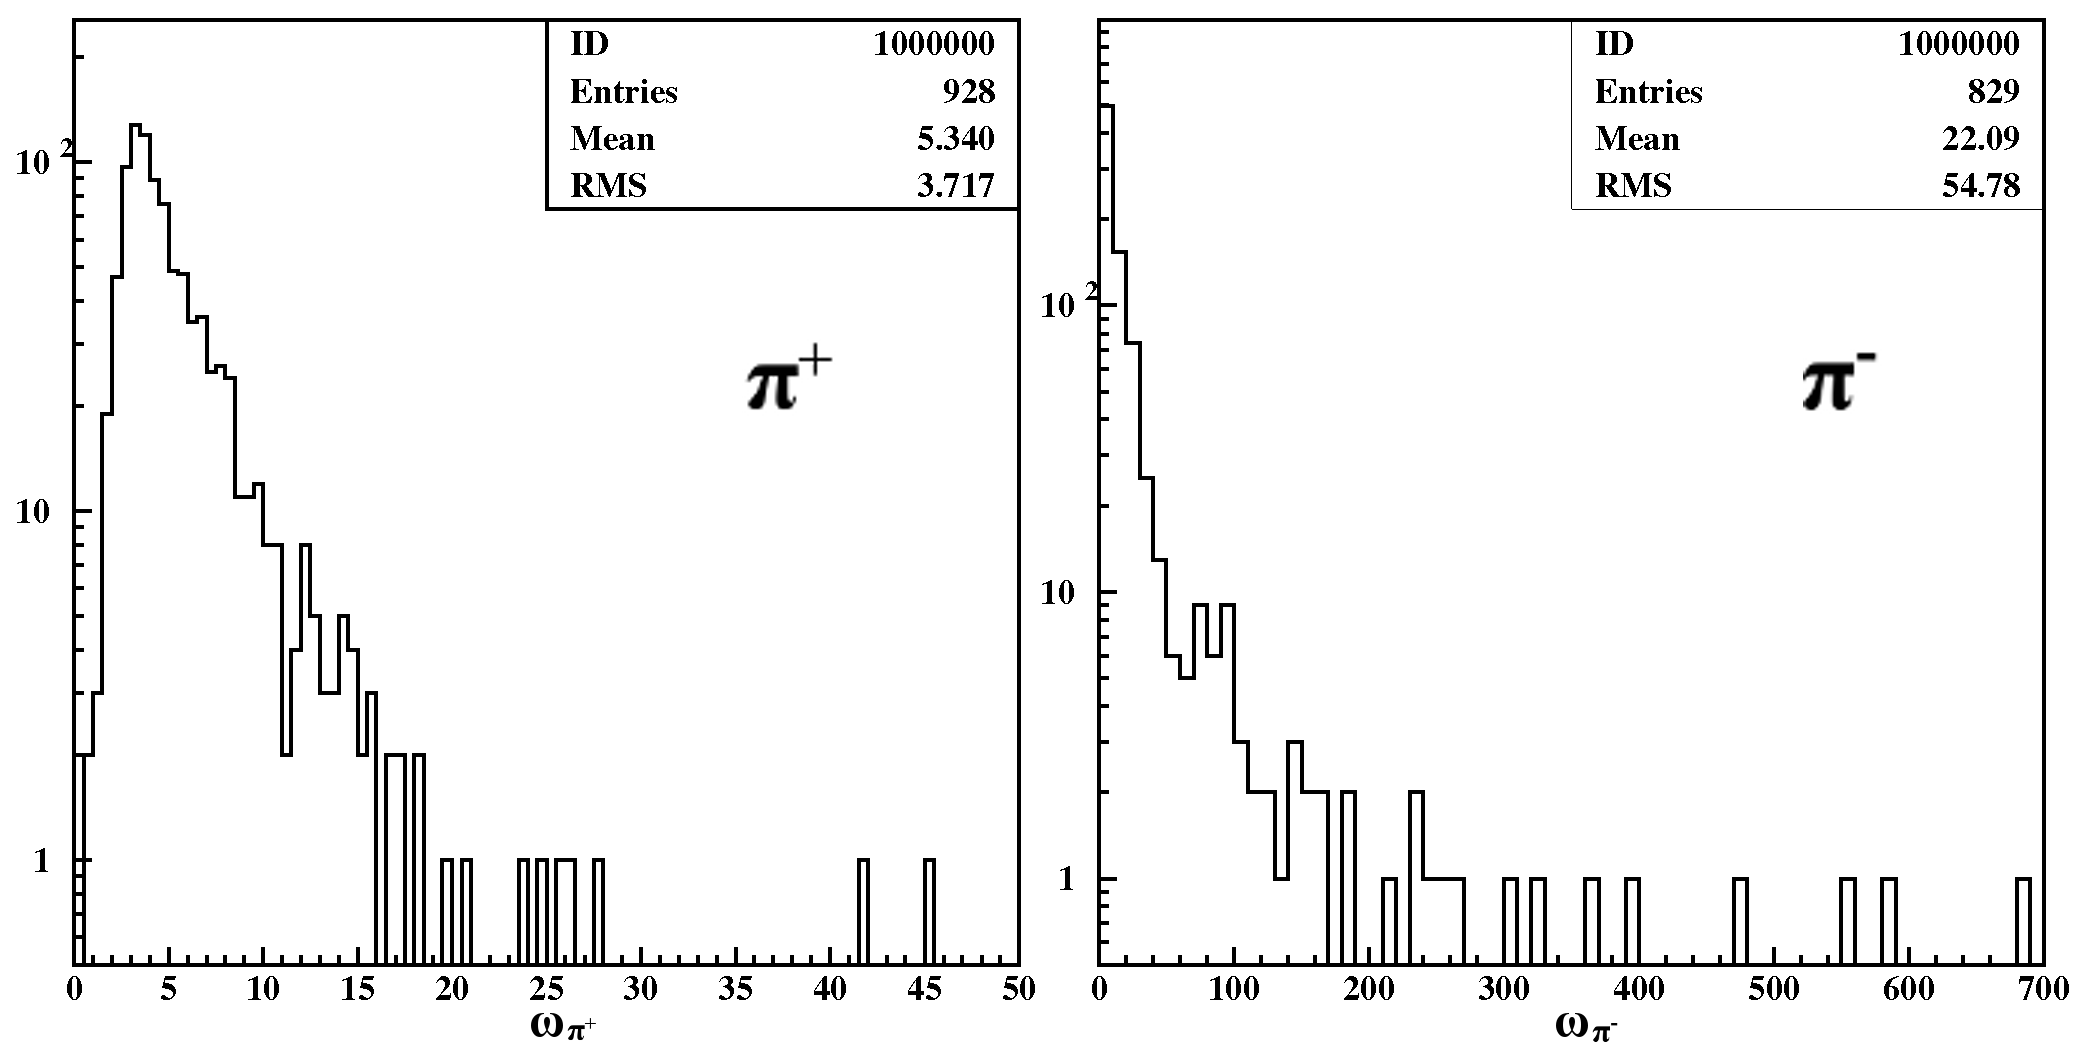
\includegraphics[width=14cm] {chap5-fig/pawpipdeut.png}
\caption {Acceptance weights for pions in deuterium (not reweighted).}
\label{fig:AccCoef}
\end{figure}

The electron acceptance, necessary in order to correct the number of electrons 
in the multiplicity ratios, is done with the same method than in the 
semi-inclusive case, but only using the two first dimensions ($\nu$ 
and $Q^2$). It is also interesting to note that no reweighting is necessary 
for electrons as all non-empty bins pass the cuts \ref{eq:AccL1} and 
\ref{eq:AccL2}.

\begin{figure}[tbp]
\centering
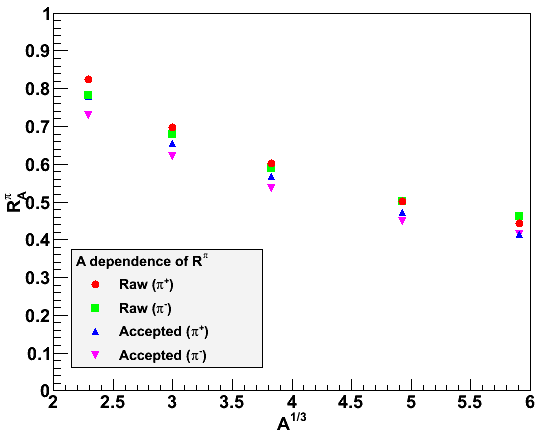
\includegraphics[width=7.4cm] {chap5-fig/b_RvA.png} 
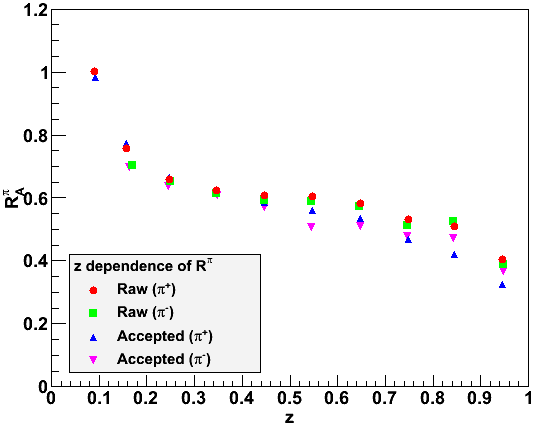
\includegraphics[width=7.4cm] {chap5-fig/b_RvZ.png} 
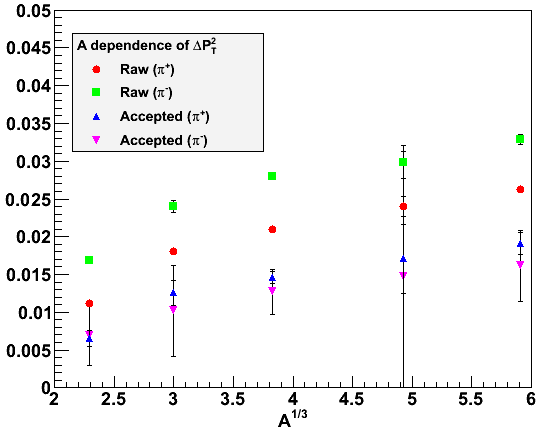
\includegraphics[width=7.4cm] {chap5-fig/b_PvA.png} 
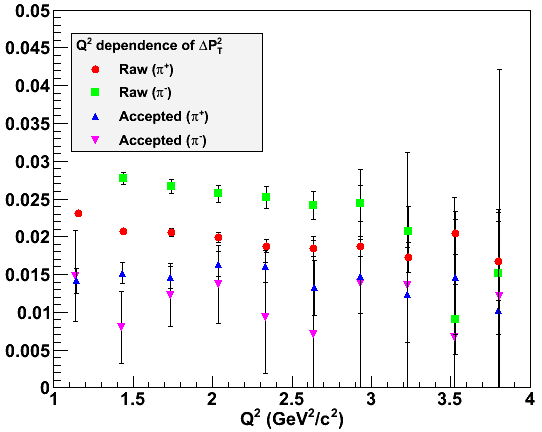
\includegraphics[width=7.4cm] {chap5-fig/b_PvQ2.png} 
\caption {Preliminary results are compared with results corrected for 
acceptance, for multiplicity ratios (top) and transverse momentum broadening 
(bottom). Only statistical errors are shown.}
\label{fig:AcceptPlots}
\end{figure}

Figure \ref{fig:AcceptPlots}, where only statistical errors are 
represented, shows the new results after applying the acceptance correction.
The acceptance effects appear to be of $\sim 10$\% for multiplicity ratios and 
$\sim 30$\% for transverse momentum broadening. This is a surprisingly 
significant correction for the few centimeters between the two targets. The 
$\pi^-$s are more affected because of CLAS' magnetic field. Indeed, the low \pt
$\pi^-$s have very low acceptance, this makes the errors 
on \dpt very large and the related results difficult to exploit. Finally, because 
of some difference in position between the solid targets (table 
\ref{tab:targets}), some extra simulation is needed in order to exploit 
correctly the aluminum and tin results. Therefore, these two targets should not be considered for 
the final results.

\subsubsection{Coulomb Correction}
\label{CCor}

The large charge of the nuclear targets create an electric field that should 
be accounted for at our energies. This nuclear electric field accelerate or 
decelerate the incoming and outgoing charged particles, it also has non 
trivial effects such as focussing effects at lower energies. Aste {\it et 
al.}~\cite{Aste:2005wc} have shown that an effective momentum approximation is 
reliable for larger momentums ($Q^2>.5$ GeV$^2$). Being clearly beyond this 
limit and the Coulomb correction being relatively small in our kinematic, we 
decide to use such an approximation. Following the prescription from Aste 
{\it et al.} we use an effective potential $\bar V= 0.8 V_0$, that they found 
best suited when using such approximation. $V_0$ being the electrostatic 
potential in the center of the nuclei, {\it i.e.}: $V_0= -3 \alpha_{EM} Z / 
(2 R)$. Values for $V_0$ and $\bar V$ used in this analysis are given in 
table~\ref{tab:Coulomb}. Coulomb corrections are applied on electrons, and
both charged pions before to calculate the kinematic variables.

\begin{table}[htbp]
  \centering
  \begin{tabular}{@{} ccc @{}}
    \hline
Nucleus & $V_0$ (MeV)  &  $\bar V$ (MeV) \\ \hline
$^2$H  & -1  &     -1 \\
C   &  -4 &      -3 \\
Al  &  -7 &      -6 \\
Fe  & -11 &    -9 \\
Sn  & -17 &   -14 \\
Pb  & -23 &   -19 \\
    \hline
  \end{tabular}
  \caption{Values for $V_0$ and $\bar V$ used for Coulomb correction of charged particles.}
  \label{tab:Coulomb}
\end{table}


\subsubsection{Radiative Correction}
\label{RadCor}

Despite its lower magnitude, compared to the strong force, the 
electromagnetic force might have a non negligible impact on our results. The 
reason is that even a moderate energy photon 
emission can modify significantly the measured kinematic variables.
To correct this effect, several simulation codes exist \cite{Akushevich:2001yp}, 
however, none permit to treat directly semi-inclusive DIS on nuclei. In order 
to make the correction, a dedicated Monte-Carlo simulation, based on existing 
codes, was developed.

\paragraph{Simulation}

The inclusive radiative effects are generated using the RADGEN software 
\cite{Akushevich:1998ft}, which includes the Feynman diagrams shown in 
figure~\ref{fig:FDRadCorr}. This code evaluates directly the correction 
factors ($\delta = \sigma_{obs} / \sigma_{Born}$) to apply for inclusive 
measurements. As RADGEN is also a Monte-Carlo generator of photon emissions, 
it can be used to modify the virtual photon kinematic before the 
hadron production in any DIS generator. This allows to evaluate the radiative 
effects on semi-inclusive measurements by implementing RADGEN inside a full 
Monte-Carlo event generator.

\begin{figure}[htbp]
\centering
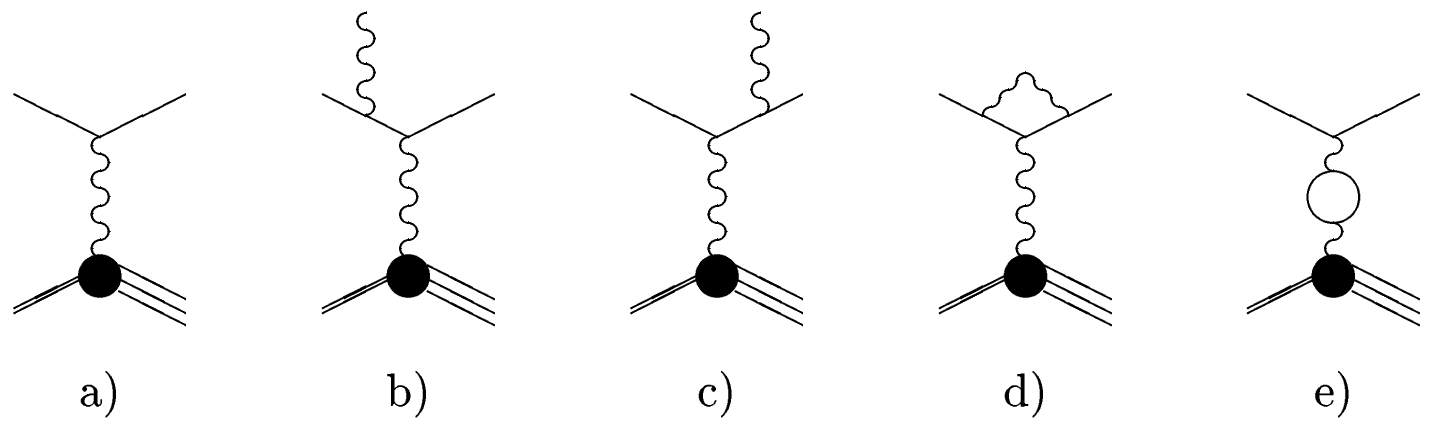
\includegraphics[width=12cm] {chap5-fig/RadDiag.png}
\caption {Diagrams taken into account in RADGEN \cite{Akushevich:1998ft}. The 
diagrams b) to e) contribute to the first order calculation of the radiative 
effects on Born cross section (diagram a)).}
\label{fig:FDRadCorr}
\end{figure}

The Monte-Carlo simulation we use is the GENIE software 
\cite{Andreopoulos:2009rq}, which describes well electron-nuclei scattering. 
Indeed, GENIE includes quasi-elastic scattering\footnote{Elastic 
scattering on a single nucleon of a nuclei.}, which is the main channel contributing 
to the radiative events in the DIS region \cite{Akushevich:2007jc}. The GENIE 
software includes also hadron cascades in the nuclei, which lead to the 
possibility to generate pions in quasi-elastic events. This is an important 
feature because the quasi-elastic cannot contribute directly to semi-inclusive 
measurements.

\paragraph{Correction of the Data}

We generate 100 million events per target, with and without radiative effects.
The RADGEN software gives direct indication for the inclusive correction and 
the comparison between the two data sets allows to extract factors for 
semi-inclusive correction.

The correction factors for inclusive ratio (figure \ref{fig:RadCorrFac}) are 
relatively small (couple of percents maximum) except at low \xb and high $\nu$. Semi-inclusive factors are 
shown in figure \ref{fig:RadCorrFacSIDIS} as a function of $z$ and \ptp. However 
the statistical error on these is large, the problem being that only a small 
fraction of the events involved photon radiation.

\begin{figure}[htbp]
\centering
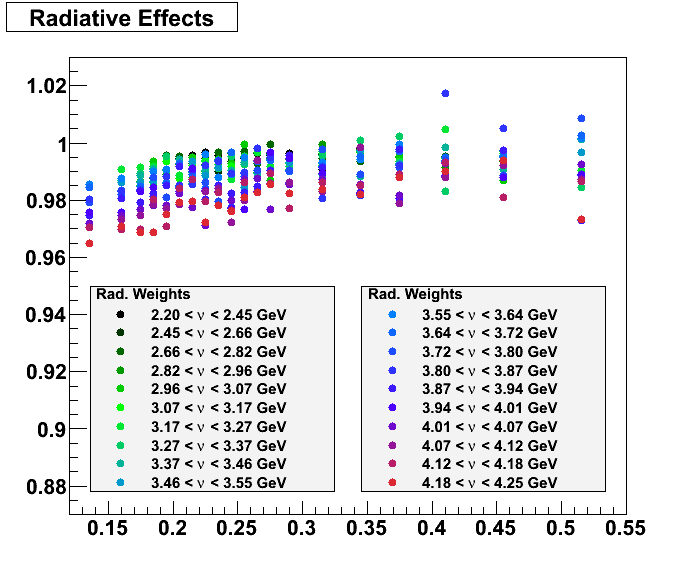
\includegraphics[width=9cm] {chap5-fig/ElecRadWei_Lead.png}
\caption {Ratios of the radiative correction factors $\delta_\text{Pb}/
\delta_{^2\text{H}}$ as a function of \xb in various $\nu$ bins.}
\label{fig:RadCorrFac}
\end{figure}

\begin{figure}[htbp]
\centering
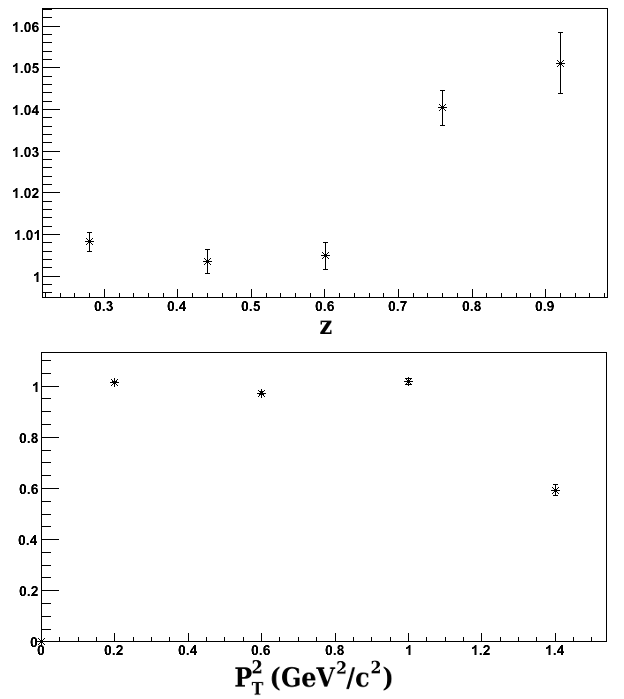
\includegraphics[width=9cm] {chap5-fig/RadGenFactors.png}
\caption {Ratios of the radiative correction factors $\delta_\text{Pb}/
\delta_{^2\text{H}}$ as a function of $z$ and \ptp.}
\label{fig:RadCorrFacSIDIS}
\end{figure}

The radiative correction appears to be limited in amplitude in most of the 
kinematic, so we decided not to apply it before further studies. Improvement can 
be easily obtained by generating more statistics, in order to analyze the 
semi-inclusive effects in more depth. Also radiative effects from the target thickness 
are ignored in the current setup; these need to be evaluated and, eventually, 
corrected as well.

\subsubsection{Isospin Correction}

The important excess of neutron in heavy nuclei leads to a modification of the 
$\pi$ multiplicity per DIS events. Using Hall~C results 
\cite{Asaturyan:2011mq}, shown in figure \ref{fig:IsoSpin}, we evaluate 
correction factors for this effect. Our simple estimation is solely based on 
proton and neutron numbers; the results for $\pi^+$s are shown in 
table~\ref{tab:isospin}. The effect on $\pi^-$ is found to be coherent with zero,
therefore no correction is applied for them. 
We attribute errors of 10\% of the effect for the isospin correction, this is chosen 
relatively to the precision of the Hall~C measurement.

\begin{figure}[tbp]
\centering
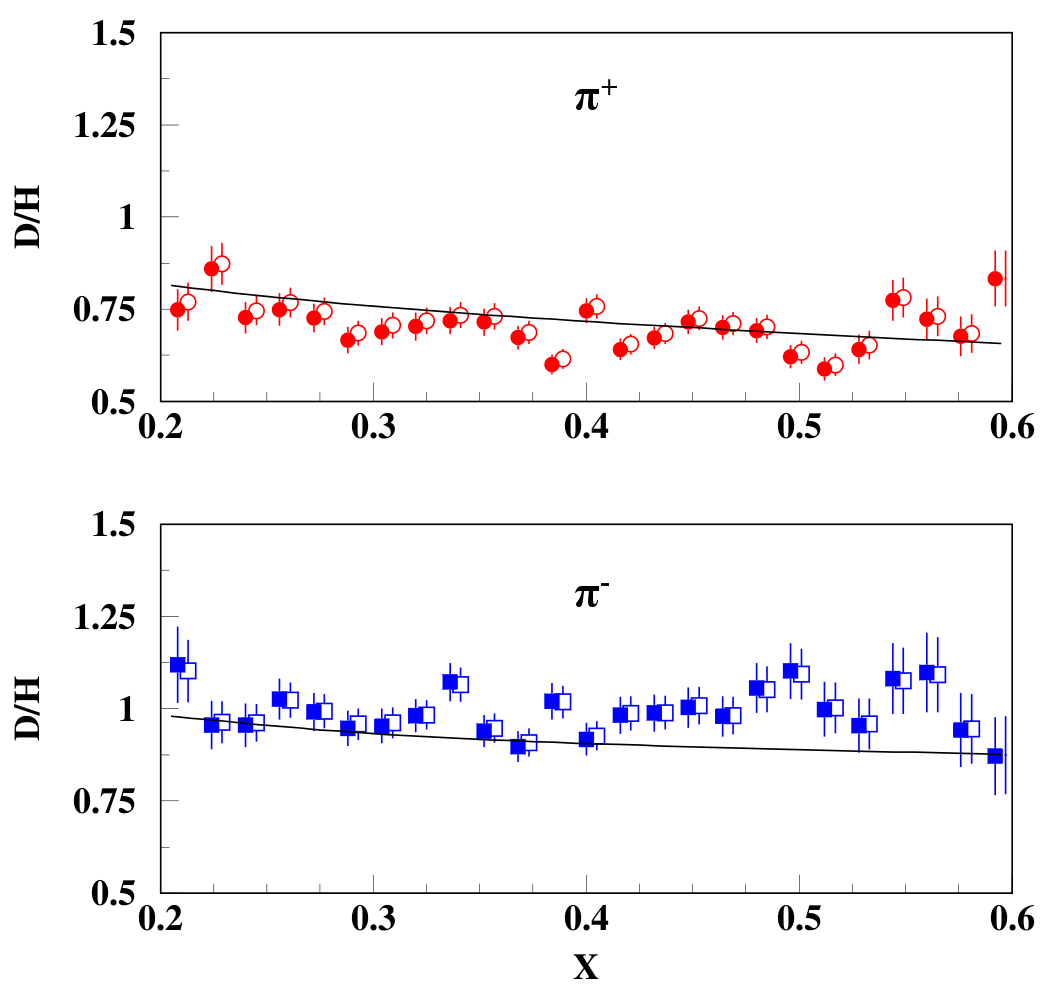
\includegraphics[width=10cm] {chap5-fig/HallC-Isospin.png}
\caption {Ratios of deuteron over proton for $\pi^+$s and $\pi^-$s 
as a function of \xb at $z=0.55$ \cite{Asaturyan:2011mq}.}
\label{fig:IsoSpin}
\end{figure}

\begin{table}[htbp]
  \centering
  \begin{tabular}{@{} cc @{}}
    \hline
    Target & Isospin  \\ 
           & correction \\ 
    \hline
    C & 0 \\
    Al & 1.5\%\\
    Fe &  3\% \\
    Sn &  8\%\\
    Pb &  10\% \\
    \hline
  \end{tabular}
  \caption{Isospin correction applied to the $\pi^+$ multiplicity ratios for different targets.}
  \label{tab:isospin}
\end{table}

It is important to note that we correct isospin effects only for rates, thus 
we correct only the multiplicity ratios. Transverse momentum broadening could, in 
principle, also be affected, however, the results from \cite{Asaturyan:2011mq} 
show no isospin effect in \ptp. This gives good confidence that \dpt is not 
affected by isospin effects.

We finally note that the $A$ dependencies of the multiplicity ratios of the 
charged pions are similar after the isospin correction\footnote{Within 
normalization errors presented in section \ref{sec:TotSys}} (figure 
\ref{fig:IsoPlot}). Considering previous measurements and existing models, 
this result was expected and confirm the need for this correction to be applied.

\begin{figure}[tbp]
\centering
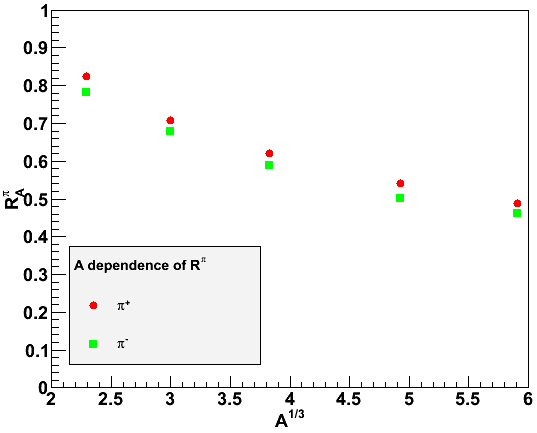
\includegraphics[width=8cm] {chap5-fig/c_RvA.png}
\caption {Multiplicity ratios as a function of $A^{1/3}$ 
with only isospin correction applied.}
\label{fig:IsoPlot}
\end{figure}

\subsection{Systematic Uncertainties}
\label{sec:TotSys}

In this section are summarized the systematic errors that we identified. The 
systematic point to point errors are calculated bin by bin for each results.
They are caused by uncertainties on the acceptance and on the identification of 
particles. The normalization errors are attributed globally. They are due to 
acceptance effects, target misidentifications and isospin correction.

\subsubsection{Quality of the Detection}
\label{SysId}

The simulation of the CLAS detector, using GSIM package, is used 
to evaluate the systematic errors linked with:

  - experimental resolution of kinematic variables,

  - particle misidentification,

  - particle re-scattering in the detector,

  - particle energy loss.\\


To evaluate those errors, we compare the reconstructed particles with the 
generated ones. Each reconstructed particle is associated with its generated parent using the
similarity in momentum and angle.
Distributions of $\Delta p$, $\Delta \theta$ and $\Delta \phi$ are defined as 
$\Delta x = {\sum_n |x_{gen} - x_{rec}| \over n}$. They give the precision with which we measure 
these variables. Using the same simulation than for the acceptance, we find 
${\delta p \over p } = 0.03$, $\delta \theta = 3$ mrad and 
$\delta \phi = 10$~mrad. These are broader than announced in \cite{Mecking:2003zu} 
but still reasonable. Then associated systematic errors can be easily 
evaluated for other variables: $\delta Q^2 \sim 0.013$ GeV$^2$/c$^2$, $\delta z \sim 
0.4 \%$, $\delta P_\perp^2 \sim 0.004$ GeV$^2$/c$^2$ and so on\footnote{These were 
evaluated for typical kinematics, the results can be significantly larger at 
extreme kinematics (large \pt or Q$^2$).}. These are negligible because they are 
several times smaller than our usual bin sizes (see figures in section 
\ref{prelim}). 

We also evaluate particle misidentification and particles originating from 
scattering in the detector or the coils. Only tails of distributions can lead to high 
contamination by misidentification, the most problematic being the tail of the 
\pt distribution. This effect is due to the low probability to produce high 
\pt events, therefore the contribution from accidental is relatively 
increased. We use the following cut $p_\perp^2 < 2.5$~GeV$^2$/c$^2$, which 
only removes a very little amount of data ($\sim 1$ $\pi$ in 30000). The 
misidentification of electrons is found to be of the order of 1 in a 1000 and 
does not contribute significantly to the uncertainty. For pions, the main 
contamination comes from kaons above 2~GeV/c ($\sim$3\% of $\pi^+$ and 
$\sim$0.5\% of $\pi^-$). Incidentally, protons also contaminates $\pi^+$ at 
high momentum (up to few \%). The uncertainty related to 
misidentification is taken into account for the point to point systematic error 
evaluation, other effects are found to be negligible.

\subsubsection{Target Reconstruction}

Because of reconstruction errors or scattering on the detector materials, it 
is possible to associate a particle with the wrong target. To estimate this 
effect, we look, in the experimental data, at the number of events 
reconstructed upstream and downstream of the targets, where nothing should be
detected. We define two test regions (see figure \ref{fig:targetleak}) to evaluate
the contamination. The region 1 is upstream and chosen to be of the same size as the window used for solid 
target selection. We use it to evaluate contamination from the liquid target to the solid one. The region 2
is downstream and of the size of the window for the liquid target selection and allows to evaluate the solid target leak into the liquid one
The distance between detection and test regions is identical to the 
distance between the two detection regions. 

We find
that the number of electrons in the test regions 1 and 2 represent 1 and 2\%, 
respectively, of the total number of events. In the case of semi-inclusive measurement, where we request
2 particles in the final state, the number drops drastically and is of the order of
0.01\%. In conclusion, only the number of electron is significantly affected by this problem
leading to a normalization error of 1\% for all multiplicity ratios.

\begin{figure}[tbp]
\centering
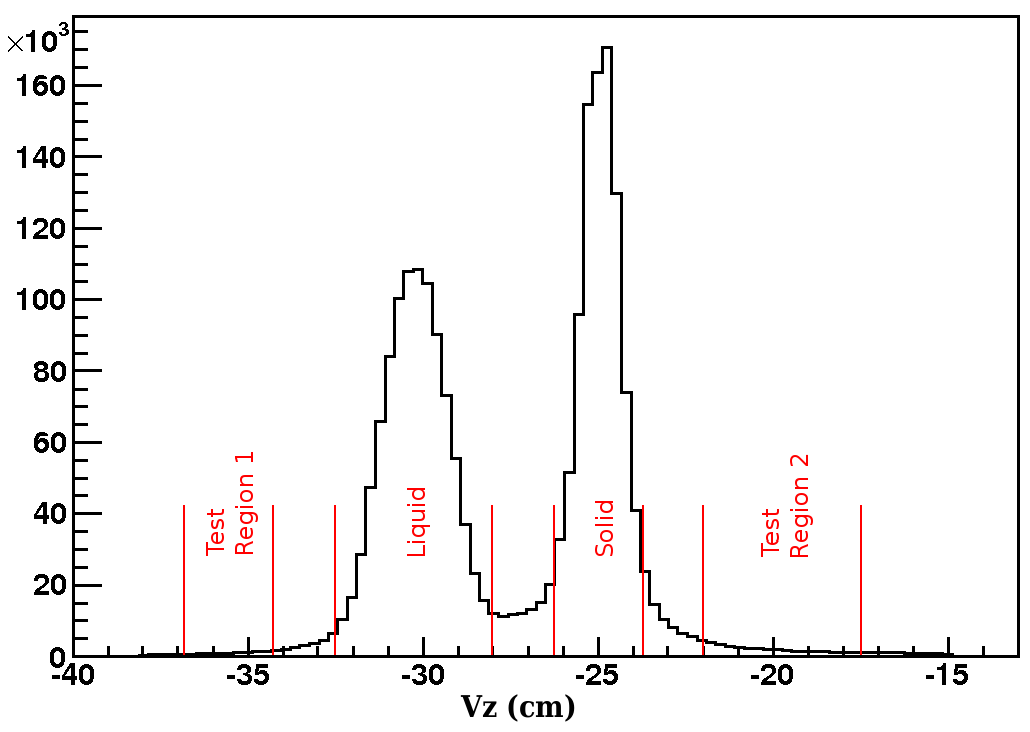
\includegraphics[width=9cm] {chap5-fig/Vertex.png}
\caption {Distribution of the vertex positions along z (cm), i.e. along the 
beam line. In red are shown the cuts used to evaluate the leak from one target to 
another.}
\label{fig:targetleak}
\end{figure}

\subsubsection{Acceptance}

We apply two different acceptance corrections to the data using two different binnings 
(table \ref{tab:AcceptBinning}). The differences between them give us a good 
indication on the systematic error associated with the method. Using a sample 
of results from iron, we find the systematic presented in the table 
\ref{tab:SysAcc}. We note the significantly larger errors for $\pi^-$, which 
was expected because of the smaller acceptance and the larger weights. More 
significant are the large errors on the \dpt measurements, this is mainly due to 
the nature of the observable; as a difference \dpt enhances relative errors 
significantly. As was seen in figure~\ref{fig:AcceptPlots}, error bars are much 
larger for corrected \dpt indicating an important statistical 
sensitivity introduced by the weighting. The errors on \dpt are of the same 
order, or smaller, as the differences observed between the two sets. This is 
an indication that the uncertainties reported in table \ref{tab:SysAcc} are already 
taken into account in the statistical error.

\begin{table}[htbp]
  \centering
\renewcommand{\arraystretch}{1.3}
  \begin{tabular}{|c|c|c|}
    \hline
    Variable & Normalization & Point to point \\ 
             & errors        & errors         \\ 
    \hline
    $R^{\pi^+}_A$  & 1.2\% & 1.5\%  \\
    $R^{\pi^-}_A$  & 2.5\% & 2.6\%   \\
    $\langle \Delta P_\perp^2 \rangle^{\pi^+}_A$ & 5\% & 11\% \\
    $\langle \Delta P_\perp^2 \rangle^{\pi^-}_A$ & 5\% & 21\% \\
    \hline
  \end{tabular}
  \caption{Relative errors on observables between the two weighting 
  described in the text.}
  \label{tab:SysAcc}
\end{table}

\subsubsection{Normalization Error}

The normalization errors -- i.e. independent of kinematic variables -- are due to acceptance effects, target identification 
and isospin correction. They are summarized in the table \ref{tab:sysid}. 

\begin{table}[htbp]
  \centering
\renewcommand{\arraystretch}{1.3}
  \begin{tabular}{|c|cc|cc|}
    \hline
              & $R_A^{\pi^+}$  & $R_A^{\pi^-}$ & \dptp$^{\pi^+}$ &  \dptp$^{\pi^-}$\\ 
    \hline
    Acceptance & 1.2\% & 2.5\% & 5\% & 5\% \\
    Target id. & 1\% & 1\% & 1\% & 1\% \\
    Isospin (Pb)& 1\% & 1\% & 1\% & 1\% \\
    Total      & 1.9\% & 2.9\% & 5.2\% & 5.2\% \\
    \hline
  \end{tabular}
  \caption{Normalization uncertainties.}
  \label{tab:sysid}
\end{table}

